\ifdefined\maindoc\else
% typesetting this chapter as a standalone document
\def\doctitle{Mechanical Models II}
% starting definitions for both the main document and stand-alone chapters
\documentclass{book}

\def\mech{artisynth.core.mechmodels}
\def\mgeo{maspack.geometry}

% Add search paths for input files
\makeatletter
\def\input@path{{../}{../../}{../texinputs/}}
\makeatother

\usepackage{amsmath}
\usepackage{framed}
%%
%% Default settings for artisynth
%%
\NeedsTeXFormat{LaTeX2e}
%%\ProvidesPackage{artisynthDoc}[2012/04/05]

\usepackage[T1]{fontenc}
\usepackage[latin1]{inputenc}
\usepackage{listings}
\usepackage{makeidx}
\usepackage{latexml}
\usepackage{graphicx}
\usepackage{framed}
\usepackage{booktabs}
\usepackage{color}

\newcommand{\pubdate}{\today}
\newcommand{\setpubdate}[1]{\renewcommand{\pubdate}{#1}}
\newcommand{\code}[1]{{\tt #1}}

\iflatexml
\usepackage{hyperref}
\setlength\parindent{0pt} 
\else
%% then we are making a PDF, so include things that LaTeXML can't handle: 
%% docbook style, \RaggedRight
\usepackage{ifxetex}
\usepackage{xstring}
\usepackage{pslatex} % fixes fonts; in particular sets a better-fitting \tt font

\usepackage[most]{tcolorbox}
\definecolor{shadecolor}{rgb}{0.95,0.95,0.95}
\tcbset{
    frame code={}
    center title,
    left=0pt,
    right=0pt,
    top=0pt,
    bottom=0pt,
    colback=shadecolor,
    colframe=white,
    width=\dimexpr\textwidth\relax,
    enlarge left by=0mm,
    boxsep=0pt,
    arc=0pt,outer arc=0pt,
}%

\usepackage[A4]{artisynth_papersize}
%\usepackage[letter]{artisynth_papersize}
\usepackage[hyperlink]{asciidoc-dblatex} 

%\usepackage{verbatim}
\usepackage{ragged2e}
\setlength{\RaggedRightRightskip}{0pt plus 4em}
\RaggedRight
\renewcommand{\DBKpubdate}{\pubdate}
\renewcommand{\DBKreleaseinfo}{}
\fi

% set hypertext links to be dark blue:
\definecolor{darkblue}{rgb}{0,0,0.8}
\definecolor{sidebar}{rgb}{0.5,0.5,0.7}
\hypersetup{colorlinks=true,urlcolor=darkblue,linkcolor=darkblue,breaklinks=true}

%%%%%%%%%%%%%%%%%%%%%%%%%%%%%%%%%%%%%%%%%%%%%%%%%%%%%%%%%%%%%%%%%%%%%%%%%%%%%
%
% Define macros for handling javadoc class and method references
%
%%%%%%%%%%%%%%%%%%%%%%%%%%%%%%%%%%%%%%%%%%%%%%%%%%%%%%%%%%%%%%%%%%%%%%%%%%%%%
\makeatletter

% macro to enable line break if inside a PDF file
\def\pdfbreak{\iflatexml\else\\\fi}

% code inspired by http://stackoverflow.com/questions/2457780/latex-apply-an-operation-to-every-character-in-a-string
\def\removeargs #1{\doremoveargs#1$\wholeString\unskip}
\def\doremoveargs#1#2\wholeString{\if#1$%
\else\if#1({()}\else{#1}\taketherest#2\fi\fi}
\def\taketherest#1\fi
{\fi \doremoveargs#1\wholeString}

% Note: still doesn't work properly when called on macro output ...
% i.e., \dottoslash{\concatnames{model}{base}{foo}} fails 
\def\dottoslash #1{\dodottoslash#1$\wholeString\unskip}
\def\dodottoslash#1#2\wholeString{\if#1$%
\else\if#1.{/}\else{#1}\fi\dottaketherest#2\fi}
\def\dottaketherest#1\fi{\fi \dodottoslash#1\wholeString}

\def\hashtodot #1{\dohashtodot#1$\wholeString\unskip}
\def\dohashtodot#1#2\wholeString{\if#1$X%
\else\if#1\#{.}\else{#1}\fi\hashtaketherest#2\fi}
\def\hashtaketherest#1\fi{\fi \dohashtodot#1\wholeString}

%\dollartodot{#1} does the same thing as \StrSubstitute[0]{#1}{\$}{.}
% from the packahe xstring. We define \dollartodot instead because
% LaTeXML does not implement xstring.
%
% Note that for the substituion to work, we need \ifx instead of \if,
% since otherwise escaped characters won't work properly:
% if #1 = \$, then \if#1* seems to compare '\' and '$' (and output '*'),
% rather than comparing '$' to '*'
\def\dollartodot #1{\dodollartodot#1*\wholeString\unskip}
\def\dodollartodot#1#2\wholeString{\ifx#1*%
\else \ifx#1\${.}\else{#1}\fi\dollartaketherest#2\fi}
\def\dollartaketherest#1\fi{\fi \dodollartodot#1\wholeString}

% concatenates up to three class/method names together, adding '.' characters
% between them. The first and/or second argument may be empty, in which case
% the '.' is omitted. To check to see if these arguments are empty, we
% use a contruction '\if#1@@', which will return true iff #1 is empty
% (on the assumption that #1 will not contain a '@' character).
\def\concatnames
#1#2#3{\if#1@@\if#2@@#3\else #2.#3\fi\else\if#2@@#1.#3\else#1.#2.#3\fi\fi}

\newcommand{\javabase}{}
\newcommand{\setjavabase}[1]{\renewcommand{\javabase}{#1}}

\def\artisynthDocBase{@ARTISYNTHDOCBASE}

\iflatexml
\def\ifempty#1{\def\temp{#1}\ifx\temp\empty}%
\newcommand{\artisynthManual}[3][]{%
   \ifempty{#1}
      \href{@ARTISYNTHDOCBASE/#2/#2.html}{#3}%
    \else
      \href{@ARTISYNTHDOCBASE/#1/#2.html}{#3}%
    \fi
}
\else
\newcommand{\artisynthManual}[3][]{%
\href{https://www.artisynth.org/@ARTISYNTHDOCBASE/#2.pdf}{#3}}
\fi

%\href{@ARTISYNTHDOCBASE/#2/#2.html}{#3}}



\newcommand{\javaclassx}[2][]{%
% Includes code to prevent an extra '.' at the front if #1 is empty. It
% works like this: if '#1' is empty, then '#1.' expands to '.', and so 
% '\if#1..' will return true, in which case we just output '#2'.
\href{@JDOCBEGIN/\concatnames{\javabase}{#1}{#2}@JDOCEND}{#2}}
\newcommand{\javaclass}[2][]{%
\href{@JDOCBEGIN/\concatnames{}{#1}{#2}@JDOCEND}{\dollartodot{#2}}}
\newcommand{\javaclassAlt}[2]{%
\href{@JDOCBEGIN/\concatnames{}{}{#1}@JDOCEND}{#2}}

\newcommand{\javamethodArgsx}[2][]{%
\href{@JDOCBEGIN/\concatnames{\javabase}{#1}{#2}@JDOCEND}{#2}}
\newcommand{\javamethodArgs}[2][]{%
\href{@JDOCBEGIN/\concatnames{}{#1}{#2}@JDOCEND}{#2}}
\newcommand{\javamethodAlt}[2]{%
\href{@JDOCBEGIN/\concatnames{}{}{#1}@JDOCEND}{#2}}
\newcommand{\javamethodAltx}[2]{%
\href{@JDOCBEGIN/\concatnames{\javabase}{}{#1}@JDOCEND}{#2}}

\newcommand{\javamethodNoArgsx}[2][]{%
\href{@JDOCBEGIN/\concatnames{\javabase}{#1}{#2}@JDOCEND}{\removeargs{#2}}}
\newcommand{\javamethodNoArgs}[2][]{%
\href{@JDOCBEGIN/\concatnames{}{#1}{#2}@JDOCEND}{\removeargs{#2}}}

\newcommand{\javamethod}{\@ifstar\javamethodNoArgs\javamethodArgs}
\newcommand{\javamethodx}{\@ifstar\javamethodNoArgsx\javamethodArgsx}

%%%%%%%%%%%%%%%%%%%%%%%%%%%%%%%%%%%%%%%%%%%%%%%%%%%%%%%%%%%%%%%%%%%%%%%%%%%%%
%
% Define macros for sidebars
%
%%%%%%%%%%%%%%%%%%%%%%%%%%%%%%%%%%%%%%%%%%%%%%%%%%%%%%%%%%%%%%%%%%%%%%%%%%%%%

\iflatexml
\newenvironment{sideblock}{\begin{quote}}{\end{quote}}
\else
\usepackage[strict]{changepage}
\definecolor{sidebarshade}{rgb}{1.0,0.97,0.8}
\newenvironment{sideblock}{%
    \def\FrameCommand{%
    \hspace{1pt}%
    {\color{sidebar}\vrule width 2pt}%
    %{\vrule width 2pt}%
    {\color{sidebarshade}\vrule width 4pt}%
    \colorbox{sidebarshade}%
  }%
  \MakeFramed{\advance\hsize-\width\FrameRestore}%
  \noindent\hspace{-4.55pt}% disable indenting first paragraph
  \begin{adjustwidth}{}{7pt}%
  %\vspace{2pt}\vspace{2pt}%
}
{%
  \vspace{2pt}\end{adjustwidth}\endMakeFramed%
}
\fi

\iflatexml
\newenvironment{shadedregion}{%
  \definecolor{shadecolor}{rgb}{0.96,0.96,0.98}%
  \begin{shaded*}%
% Put text inside a quote to create a surrounding blockquote that
% will properly accept the color and padding attributes
  \begin{quote}%
}
{%
  \end{quote}%
  \end{shaded*}%
}
\else
\newenvironment{shadedregion}{%
  \definecolor{shadecolor}{rgb}{0.96,0.96,0.98}%
  \begin{shaded*}%
}
{%
  \end{shaded*}%
}
\fi

% Wanted to create a 'listing' environment because lstlisting is
% tedious to type and because under latexml it may need
% some massaging to get it to work properly. But hard to do
% because of the verbatim nature of listing
%\iflatexml
%\newenvironment{listing}{\begin{lstlisting}}{\end{lstlisting}}%
%\else
%\newenvironment{listing}{\begin{lstlisting}}{\end{lstlisting}}%
%\fi

\iflatexml\else
% fancyhdr was complaining that it wanted a 36pt header height ...
\setlength{\headheight}{36pt}
\fi

% macro for backslash character
\newcommand\BKS{\textbackslash}

% macro for double hyphen (to prevent conversion of -- into -)
\newcommand\DHY{-{}-}

% Convenience stuff
\newcommand{\ifLaTeXMLelse}[2]{%
  \iflatexml %
  #1 %
  \else %
  #2 %
  \fi %
}

\newcommand{\ifLaTeXML}[1]{ %
  \iflatexml %
  #1 %
  \fi %
}

% new methodtable environment for documenting methods

% base width of the method table
\newlength{\methodtablewidth}
\iflatexml
\setlength{\methodtablewidth}{1.4\textwidth}
\else
\setlength{\methodtablewidth}{0.94\textwidth}
\fi
% horizontal space added at end of call to \methodentry
\newlength{\methodskip}
\setlength{\methodskip}{0pt}
% lengths set inside methodtable environment:
\newlength{\methodsiglength} % length of the method signature
\newlength{\methodcomlength} % length of the method comment
\setlength{\methodsiglength}{0.5\methodtablewidth}
\setlength{\methodcomlength}{0.5\methodtablewidth}

% command to add a method to a method table:
% arg #1: package and signature for finding URL
% arg #2: anchor text
% arg #3: comment describing the method
\newcommand{\methodentry}[3]{%
\javamethodAlt{#1}{\parbox[t]{\methodsiglength}{#2}}&
{\parbox[t]{\methodcomlength}{#3}}\\%
\noalign{\vspace{\methodskip}}}

% methodtable environment takes two arguments, both scale factors for
% methodtablewidth:
% arg #1: width of the method signature column
% arg #2: width of the method comment column
\newenvironment{methodtable}[3][0pt]{%
\begingroup
\setlength{\topskip}{0pt}
\setlength{\methodskip}{#1}
\setlength{\methodsiglength}{#2\methodtablewidth}%
\setlength{\methodcomlength}{#3\methodtablewidth}%
\iflatexml
\begin{snugshade}
\else
\begin{tcolorbox}
\fi
\renewcommand{\arraystretch}{1}
\begin{tabular}{ll}}{%
\end{tabular}
\renewcommand{\arraystretch}{1}
\iflatexml
\end{snugshade}
\else
\end{tcolorbox}
\fi
\endgroup}

% commands for added top, mid and bottom lines in the table.
% uses booktabs for PDF, regular hline for HTML
\newcommand{\topline}{\iflatexml\hline\else\toprule\fi}
\newcommand{\midline}{\iflatexml\hline\else\midrule\fi}
\newcommand{\botline}{\iflatexml\hline\else\bottomrule\fi}
\newcommand{\blankline}{%
\multicolumn{2}{l}{\iflatexml{@SPACE}\else\phantom{M}\fi}\\}%
% add vertical space within a two colum method environment
\newcommand{\methodspace}[1]{%
\iflatexml
\multicolumn{2}{l}{@VERTSPACE[#1]}\\
\else
\noalign{\vspace{#1}}%
\fi}%
% break a line and add an indentation of 1em
\newcommand{\brh}{\\\phantom{M}}

\makeatother

\def\matl{\left(\begin{matrix}}
\def\matr{\end{matrix}\right)}

\def\Bthe{\boldsymbol\theta}
\def\Btau{\boldsymbol\tau}
\def\Bom{\boldsymbol\omega}
\def\Bdel{\boldsymbol\delta}
\def\Blam{\boldsymbol\lambda}
\def\Bphi{\boldsymbol\phi}
\def\Bxi{\boldsymbol\xi}
\def\Bgam{\boldsymbol\gamma}
\def\Bsig{\boldsymbol\sigma}
\def\Bnu{\boldsymbol\nu}
\def\Bmu{\boldsymbol\mu}

\def\A{{\bf A}}
\def\B{{\bf B}}
\def\C{{\bf C}}
\def\D{{\bf D}}
\def\F{{\bf F}}
\def\G{{\bf G}}
\def\H{{\bf H}}
\def\I{{\bf I}}
\def\J{{\bf J}}
\def\K{{\bf K}}
\def\Jc{{\bf J}_c}
\def\L{{\bf L}}
\def\M{{\bf M}}
\def\N{{\bf N}}
\def\O{{\bf O}}
\def\P{{\bf P}}
\def\Q{{\bf Q}}
\def\R{{\bf R}}
\def\T{{\bf T}}
\def\U{{\bf U}}
\def\W{{\bf W}}
\def\X{{\bf X}}
\def\Minv{{\bf M}^{-1}}

\def\a{{\bf a}}
\def\b{{\bf b}}
\def\c{{\bf c}}
\def\d{{\bf d}}
\def\e{{\bf e}}
\def\f{{\bf f}}
\def\g{{\bf g}}
\def\k{{\bf k}}
\def\l{{\bf l}}
\def\m{{\bf m}}
\def\n{{\bf n}}
\def\p{{\bf p}}
\def\q{{\bf q}}
\def\r{{\bf r}}
\def\u{{\bf u}}
\def\v{{\bf v}}
\def\w{{\bf w}}
\def\x{{\bf x}}
\def\y{{\bf y}}
\def\z{{\bf z}}

\def\ma{{\bf m}_\alpha}
\def\mb{{\bf m}_\beta}
\def\va{{\bf v}_\alpha}
\def\vb{{\bf v}_\beta}
\def\vp{{\bf v}_\rho}
\def\vk{{\bf v}_k}
\def\ua{{\bf u}_\alpha}
\def\ub{{\bf u}_\beta}
\def\uk{{\bf u}_k}
\def\uj{{\bf u}_j}
\def\mar{{\bf m}_{\alpha r}}
\def\mbr{{\bf m}_{\beta r}}

\def\Maa{{\bf M}_{\alpha\alpha}}
\def\Mab{{\bf M}_{\alpha\beta}}
\def\Mba{{\bf M}_{\beta\alpha}}
\def\Mbb{{\bf M}_{\beta\beta}}
\def\hatMaa{\hat{\bf M}_{\alpha\alpha}}
\def\hatMab{\hat{\bf M}_{\alpha\beta}}
\def\hatMba{\hat{\bf M}_{\beta\alpha}}
\def\hatMbb{\hat{\bf M}_{\beta\beta}}
\def\Mbp{{\bf M}_{\beta\rho}}
\def\Map{{\bf M}_{\alpha\rho}}
\def\Mpa{{\bf M}_{\rho\alpha}}
\def\Mpb{{\bf M}_{\rho\beta}}
\def\Mpp{{\bf M}_{\rho\rho}}
\def\Mbk{{\bf M}_{\beta k}}
\def\Mak{{\bf M}_{\alpha k}}
\def\Mka{{\bf M}_{k\alpha}}
\def\Mkb{{\bf M}_{k\beta}}
\def\Mkk{{\bf M}_{kk}}

\def\Ga{{\bf G}_{\alpha}}
\def\Gp{{\bf G}_{\rho}}
\def\Gaa{{\bf G}_{\alpha\alpha}}
\def\Gab{{\bf G}_{\alpha\beta}}
\def\Gba{{\bf G}_{\beta\alpha}}
\def\Gbb{{\bf G}_{\beta\beta}}
\def\Gap{{\bf G}_{\alpha\rho}}
\def\Gpa{{\bf G}_{\rho\alpha}}
\def\Gbp{{\bf G}_{\beta\rho}}
\def\Gak{{\bf G}_{\alpha k}}
\def\Gka{{\bf G}_{k\alpha}}
\def\Gja{{\bf G}_{j\alpha}}
\def\Gkb{{\bf G}_{k\beta}}
\def\Gbk{{\bf G}_{\beta k}}

\def\lama{\Blam_{\alpha}}
\def\lamb{\Blam_{\beta}}
\def\lamp{\Blam_{\rho}}
\def\lamk{\Blam_{k}}
\def\lams{\Blam_{\sigma}}

\def\ba{{\bf b}_{\alpha}}
\def\bb{{\bf b}_{\beta}}
\def\fp{{\bf f}_{\rho}}
\def\fa{{\bf f}_{\alpha}}
\def\qa{{\bf q}_{\alpha}}
\def\qb{{\bf q}_{\beta}}
\def\za{{\bf z}_{\alpha}}
\def\zb{{\bf z}_{\beta}}
\def\wa{{\bf w}_{\alpha}}
\def\wb{{\bf w}_{\beta}}

\def\Na{\bar{\bf N}_{\alpha}}
\def\Nb{\bar{\bf N}_{\beta}}

\def\Up{{\bf U}_p}
\def\Un{{\bf U}_n}

\def\dFdl{\frac{\partial F}{\partial l}}
\def\dFddl{\frac{\partial F}{\partial \dot l}}

\def\Sr{s_\theta}
\def\Cr{c_\theta}
\def\Sp{s_\phi}
\def\Cp{c_\phi}
\def\Sy{s_\psi}
\def\Cy{c_\psi}
\def\Sa{s_{\alpha}}
\def\Ca{c_{\alpha}}
\def\Vp{v_{\phi}}


\iflatexml
\else
\usepackage{biblatex}
\addbibresource{references.bib}
\fi

\setcounter{tocdepth}{5}
\setcounter{secnumdepth}{3}

\title{\doctitle}
\ifdefined\maindoc
\author{John Lloyd and Antonio S\'anchez}
\setpubdate{Last update: March, 2022}

\iflatexml
\date{}
\fi
\fi

% graphics paths
\graphicspath{{./}{images/}}

% Listings settings
\definecolor{myblue}{rgb}{0,0,0.6}
\definecolor{mygreen}{rgb}{0,0.6,0}
\definecolor{mygray}{rgb}{0.5,0.5,0.5}
\definecolor{mylightgray}{rgb}{0.95,0.95,0.95}
\definecolor{mymauve}{rgb}{0.58,0,0.82}
\definecolor{myblack}{rgb}{0,0,0}
\lstset{
   language=Java,                   % text highlighting for Java
   breakatwhitespace=false,         % automatic breaks only at whitespace
   breaklines=true,                 % automatic line breaking
   commentstyle=\color{mygreen},    % comment style
   keepspaces=true,                 % keeps spaces in text
   keywordstyle=\color{myblue},     % keyword style
   numbers=none,                    % line-numbers; values: (none, left, right)
   numbersep=5pt,                   % how far the line-numbers are from code
   numberstyle=\tiny\color{mygray}, % line-numbers style
   showspaces=false,                % show spaces everywhere
   showstringspaces=false,          % underline spaces within strings
   showtabs=false,                  % show tabs
   stepnumber=1,                    % the step between two line-numbers
   stringstyle=\color{mymauve},     % string literal style
   tabsize=3,                       % sets default tabsize to 3 spaces
   backgroundcolor=\color{mylightgray}, % background color
   frame=single, 					% adds a frame around the code
   rulesepcolor=\color{mygray},
   rulecolor=\color{myblack},
   framerule=0pt,
   xleftmargin=2.2ex,               % numbers inside box
   framexleftmargin=2.2ex,			% indentation of frame
}

\begin{document}

\frontmatter

%\layout
\maketitle

\iflatexml{\large\pubdate}\fi

\tableofcontents

\mainmatter
\fi

\def\lfn{\hat{l}_f} % normalized muscle fibre length
\def\vfn{\hat{v}_f} % normalized muscle fibre velocity
\def\ltn{\hat{l}_t} % normalized tendon length
\def\vmax{V_{m}} % max contraction velocity
\def\eps{\epsilon} % max contraction velocity
\def\Flen{\bar{F}^M_{len}} % maximum normalized lengthening force
\chapter{Mechanical Models II}
\label{MechModelsII:sec}

This section provides additional material on building basic
multibody-type mechanical models.

\section{Simulation control properties}

Both \javaclass[artisynth.core.workspace]{RootModel} and
\javaclass[artisynth.core.mechmodels]{MechModel} contain properties
that control the simulation behavior. 

\subsection{Simulation step size}

One of the most important properties is {\tt maxStepSize}. By default,
simulation proceeds using the {\tt maxStepSize} value defined for the
root model. A {\tt MechModel} (or any other type of {\tt Model})
contained in the root model's {\tt models} list may also request a
smaller step size by specifying a smaller value for its own {\tt
maxStepSize} property.  For all models, the {\tt maxStepSize} may be
set and queried using
% method table
\begin{lstlisting}[]
  void setMaxStepSize (double maxh);
  double getMaxStepSize();
\end{lstlisting}
%

\subsection{Integrator}

Another important simulation property is {\tt integrator} in {\tt
MechModel}, which determines the type of integrator used for the
physics simulation. The value type of this property is the enumerated
type {\tt MechSystemSolver.Integrator}, for which the following values
are currently defined:

\begin{description}

\item[ForwardEuler]\mbox{}

First order forward Euler integrator. Unstable for stiff systems.

\item[SymplecticEuler]\mbox{}

First order symplectic Euler integrator, more energy conserving
that forward Euler. Unstable for stiff systems.

\item[RungeKutta4]\mbox{}

Fourth order Runge-Kutta integrator, quite accurate but also unstable
for stiff systems.

\item[ConstrainedBackwardEuler]\mbox{}

First order backward order integrator. Generally stable for stiff systems.

\item[Trapezoidal]\mbox{}

Second order trapezoidal integrator. Generally stable for stiff
systems, but slightly less so than\pdfbreak
{\tt ConstrainedBackwardEuler}.

\end{description}

The term ``Unstable for stiff systems'' means that the integrator is
likely to go unstable in the presence of ``stiff'' systems, which
typically include systems containing finite element models, unless the
simulation step size is set to an extremely small value.  The default
value for {\tt integrator} is {\tt ConstrainedBackwardEuler}.

\begin{sideblock}
Stiff systems tend to arise in models containing interconnected
deformable elements, for which the step size should not exceed the
propagation time across the smallest element, an effect known as the
Courant-Friedrichs-Lewy (CFL) condition. Larger stiffness and damping
values decrease the propagation time and hence the allowable step
size.
\end{sideblock}

\subsection{Position stabilization}

Another {\tt MechModel} simulation property is {\tt stabilization},
which controls the stabilization method used to correct drift from
position constraints and correct interpenetrations due to collisions
(Chapter \ref{ContactAndCollision:sec}).
The value type of this property value is the enumerated type {\tt
MechSystemSolver.PosStabilization}, which presently has two values:

\begin{description}

\item[GlobalMass]\mbox{}

Uses only a diagonal mass matrix for the MLCP that is solved to
determine the position corrections. This is the default method.

\item[GlobalStiffness]\mbox{}

Uses a stiffness-corrected mass matrix for the MLCP that is solved to
determine the position corrections. Slower than {\tt GlobalMass}, but
more likely to produce stable results, particularly for
problems involving FEM collisions.

\end{description}

\section{Units}
\label{sec:mechii:units}

ArtiSynth is primarily ``unitless'', in the sense that it does not
define default units for the fundamental physical quantities of time,
length, and mass. Although time is
generally understood to be in seconds, and often declared as such in
method arguments and return values, there is no hard requirement that
it be interpreted as seconds. There are no assumptions at all
regarding length and mass. Some components may have default parameter
values that reflect a particular choice of units, such as {\tt
MechModel}'s default gravity value of $(0, 0, -9.8)^T$, which is
associated with the MKS system, but these values can always be
overridden by the application.

Nevertheless, it is important, and up to the application developer to
ensure, that units be {\it consistent}. For example, if one decides to
switch length units from meters to centimeters (a common choice),
then all units involving length will have to be scaled appropriately.
For example, density, whose fundamental units are $m/d^3$, where $m$ is mass and
$d$ is distance, needs to be scaled by $1/100^3$, or $0.000001$, when
converting from meters to centimeters.

Table \ref{Units:tab} lists a number of common physical quantities
used in ArtiSynth, along with their associated fundamental units.

\begin{table}
\begin{center}
\begin{tabular}{|lll|}
\hline
unit & fundamental units & \\
\hline
time                    & $t$ & \\
distance                & $d$ & \\
mass                    & $m$ & \\
velocity                & $d/t$ & \\
acceleration            & $d/t^2$ & \\
force                   & $m d/t^2$ & \\
work/energy             & $m d^2/t^2$& \\
torque                  & $m d^2/t^2$ & same as energy (somewhat counter intuitive)\\
angular velocity        & $1/t$ & \\
angular acceleration    & $1/t^2$ & \\
rotational inertia      & $m d^2$ & \\
pressure                & $m/(d t^2)$ & \\
Young's modulus         & $m/(d t^2)$ & \\
Poisson's ratio         & 1 & no units; it is a ratio \\
density                 & $m/d^3$ & \\
linear stiffness        & $m/t^2$ & \\
linear damping          & $m/t$ & \\
rotary stiffness        & $m d^2/t^2$ & same as torque \\
rotary damping          & $m d^2/t$ & \\
mass damping            & $1/t$ & used in FemModel \\
stiffness damping       & $t$ & used in FemModel \\
\hline
\end{tabular}
\end{center}
\caption{Physical quantities and their representation in terms of the
fundamental units of mass ($m$), distance ($d$), and time ($t$).}
\label{Units:tab}
\end{table}

\subsection{Scaling units}

For convenience, many ArtiSynth components, including {\tt MechModel},
implement the interface
\javaclass[artisynth.core.util]{ScalableUnits}, which
provides the following methods for scaling mass and distance units:
% method table
\begin{lstlisting}[]
  scaleDistance (s);    // scale distance units by s
  scaleMass (s);        // scale mass units by s
\end{lstlisting}
%
A call to one of these methods should cause all physical quantities
within the component (and its descendants) to be
scaled as required by the fundamental unit relationships
as shown in Table \ref{Units:tab}.

Converting a {\tt MechModel} from meters to centimeters can therefore be
easily done by calling 
%
\begin{lstlisting}[]
   mech.scaleDistance (100);
\end{lstlisting}
%
As an example, adding the following code to the end of the {\tt build()}
method in {\tt RigidBodySpring} (Section \ref{RigidBodySpringExample:sec})
%
\begin{lstlisting}[]
   System.out.println ("length=" + spring.getLength());
   System.out.println ("density=" + box.getDensity());
   System.out.println ("gravity=" + mech.getGravity());
   mech.scaleDistance (100);
   System.out.println ("");
   System.out.println ("scaled length=" + spring.getLength());
   System.out.println ("scaled density=" + box.getDensity());
   System.out.println ("scaled gravity=" + mech.getGravity());
\end{lstlisting}
%
will scale the distance units by 100 and print the values of various
quantities before and after scaling. The resulting output is:
%
\begin{lstlisting}[]
   length=0.5
   density=20.0
   gravity=0.0 0.0 -9.8

   scaled length=50.0
   scaled density=2.0E-5
   scaled gravity=0.0 0.0 -980.0
\end{lstlisting}
%

\begin{sideblock}
It is important not to confuse scaling units with scaling the actual
geometry or mass. Scaling units should change all physical
quantities so that the simulated behavior of the model remains
unchanged.  If the distance-scaled version of {\tt RigidBodySpring}
shown above is run, it should behave exactly the same as the
non-scaled version.
\end{sideblock}

\section{Render properties}
\label{RenderProperties:sec}

All ArtiSynth components that are renderable maintain a property {\tt
renderProps}, which stores a
\javaclass[maspack.render]{RenderProps} object that contains a number
of subproperties used to control an object's rendered appearance.

In code, the {\tt renderProps} property for an object can be set or
queried using the methods
% method table
\begin{lstlisting}[]
  setRenderProps (RenderProps props); // set render properties
  RenderProps getRenderProps();       // get render properties (read-only)
\end{lstlisting}
%
Render properties can also be set in the GUI by selecting one or more
components and the choosing {\sf Set render props ...}  in the
right-click context menu. More details on setting render properties
through the GUI can be found in the section ``Render properties'' in the
\artisynthManual{uiguide}{ArtiSynth User Interface Guide}.

For many components, the default value of {\tt renderProps} is {\tt
null}; i.e., no {\tt RenderProps} object is assigned by default and
render properties are instead inherited from ancestor components
further up the hierarchy. The reason for this is because {\tt
RenderProps} objects are fairly large (many kilobytes), and so
assigning a unique one to every component could consume too much
memory. Even when a {\tt RenderProps} object is assigned, most of its
properties are inherited by default, and so only those properties
which are explicitly set will differ from those specified in ancestor
components.

\subsection{Render property taxonomy}

In general, the properties in {\tt RenderProps} are used to control
the color, size, and style of the three primary rendering
primitives: faces, lines, and points. Table \ref{RenderProps:tab}
contains a complete list. Values for the {\tt shading}, {\tt
faceStyle}, {\tt lineStyle} and {\tt pointStyle} properties are
defined using the following enumerated types:
\javaclass[maspack.render]{Renderer\$Shading}, 
\javaclass[maspack.render]{Renderer\$FaceStyle}, 
\javaclass[maspack.render]{Renderer\$PointStyle}, 
and 
\javaclass[maspack.render]{Renderer\$LineStyle}.
Colors are specified using {\tt java.awt.Color}.

\begin{table}
\begin{center}
\begin{tabular}{|lll|}
\hline property & purpose & usual default value \\ \hline
%Generic properties:
visible & whether or not the component is visible & {\tt true} \\
alpha & transparency for diffuse colors (range 0 to 1) & 1 (opaque) \\
shading & shading style: 
({\tt FLAT}, {\tt SMOOTH}, {\tt METAL}, {\tt NONE}) & {\tt FLAT}\\
shininess & shininess parameter (range 0 to 128) & 32 \\
specular & specular color components & {\tt null} \\
%Face related properties &
\hline
faceStyle &
which polygonal faces are drawn ({\tt FRONT}, {\tt BACK},
{\tt FRONT\_AND\_BACK}, {\tt NONE}) & {\tt FRONT} \\
faceColor &
diffuse color for drawing faces & {\tt GRAY} \\
backColor &
diffuse color used for the backs of faces. 
If {\tt null}, {\tt faceColor} is used. & {\tt null} \\
drawEdges & hint that polygon edges should be drawn explicitly & {\tt false} \\
%Texture mapping properties &
\hline
colorMap & color mapping properties 
(see Section \ref{TextureMapping:sec}) & {\tt null} \\
normalMap & normal mapping properties 
(see Section \ref{TextureMapping:sec}) & {\tt null} \\
bumpMap & bump mapping properties 
(see Section \ref{TextureMapping:sec}) & {\tt null} \\
% Edge related properties &
\hline
edgeColor & diffuse color for edges & {\tt null} \\
edgeWidth & edge width in pixels & 1 \\
% Line related properties &
\hline
lineStyle: &
how lines are drawn ({\tt CYLINDER}, {\tt LINE}, or {\tt SPINDLE}) & 
{\tt LINE} \\
lineColor & diffuse color for lines & {\tt GRAY} \\
lineWidth & width in pixels when {\tt LINE} style is selected & 1 \\
lineRadius & radius when {\tt CYLINDER} or {\tt SPINDLE} style is selected &
1 \\
% Point related properties &
\hline
pointStyle & how points are drawn ({\tt SPHERE} or {\tt POINT}) & {\tt POINT} \\
pointColor & diffuse color for points & {\tt GRAY} \\
pointSize & point size in pixels when {\tt POINT} style is selected & 1 \\
pointRadius & sphere radius when {\tt SPHERE} style is selected & 1 \\
\hline
\end{tabular}
\end{center}
\caption{Render properties and their default values.}
\label{RenderProps:tab}
\end{table}

To increase and improve their visibility, both the line and point
primitives are associated with styles ({\tt CYLINDER}, {\tt
SPINDLE}, and {\tt SPHERE}) that allow them to be rendered using 3D
surface geometry.

Exactly how a component interprets its render properties is up to the
component (and more specifically, up to the rendering method for that
component).  Not all render properties are relevant to all components,
particularly if the rendering does not use all of the rendering
primitives. For example,
\javaclass[artisynth.core.mechmodels]{Particle} components use only
the point primitives and
\javaclass[artisynth.core.mechmodels]{AxialSpring} components use only
the line primitives. For this reason, some components use subclasses
of {\tt RenderProps}, such as
\javaclass[maspack.render]{PointRenderProps} and
\javaclass[maspack.render]{LineRenderProps}, that expose only a subset
of the available render properties. All renderable components provide
the method
\javamethod[maspack.render.HasRenderProps]{createRenderProps()} that
will create and return a {\tt RenderProps} object suitable for that
component.

\subsection{Setting render properties}
\label{SettingRenderProperties:sec}

When setting render properties, it is important to note that
the value returned by
\javamethod[maspack.render.HasRenderProps]{getRenderProps()} 
should be treated as {\it read-only} and should {\it not}
be used to set property values.
For example, applications should {\it not} do the
following:
\begin{lstlisting}[]
   particle.getRenderProps().setPointColor (Color.BLUE);
\end{lstlisting}
%
This can cause problems for two reasons. First, {\tt getRenderProps()}
will return {\tt null} if the object does not currently have a {\tt
RenderProps} object. Second, because {\tt RenderProps} objects are
large, ArtiSynth may try to share them between components, and so by
setting them for one component, the application my inadvertently set
them for other components as well.

Instead, {\tt RenderProps} provides a static method for each property
that can be used to set that property's value for a specific
component.  For example, the correct way to set {\tt pointColor} is
%
\begin{lstlisting}[]
   RenderProps.setPointColor (particle, Color.BLUE);
\end{lstlisting}
%

One can also set render properties by calling
\javamethod*[maspack.render.HasRenderProps]{setRenderProps()} with a
predefined {\tt RenderProps} object as an argument. This is useful for
setting a large number of properties at once:
%
\begin{lstlisting}[]
   RenderProps props = new RenderProps();
   props.setPointColor (Color.BLUE);
   props.setPointRadius (2);
   props.setPointStyle (RenderProps.PointStyle.SPHERE);

   ...

   particle.setRenderProps (props);
\end{lstlisting}

For setting each of the color properties within {\tt RenderProps},
one can use either {\tt Color} objects or {\tt float[]} arrays
of length 3 giving the RGB values. Specifically, there
are methods of the form
%
\begin{lstlisting}[]
   props.setXXXColor (Color color)
   props.setXXXColor (float[] rgb)
\end{lstlisting}
%
as well as the static methods
%
\begin{lstlisting}[]
   RenderProps.setXXXColor (Renderable r, Color color)
   RenderProps.setXXXColor (Renderable r, float[] rgb)
\end{lstlisting}
%
where {\tt XXX} corresponds to {\tt Point}, {\tt Line}, {\tt Face},
{\tt Edge}, and {\tt Back}. For {\tt Edge} and {\tt Back}, both {\tt
color} and {\tt rgb} can be given as {\tt null} to clear the indicated
color. For the specular color, the associated methods are
%
\begin{lstlisting}[]
   props.setSpecular (Color color)
   props.setSpecular (float[] rgb)
   RenderProps.setSpecular (Renderable r, Color color)
   RenderProps.setSpecular (Renderable r, float[] rgb)
\end{lstlisting}
%

\begin{sideblock}
Note that even though components may use a subclass of {\tt
RenderProps} internally, one can always use the base {\tt RenderProps}
class to set values; properties which are not relevant to the
component will simply be ignored.
\end{sideblock}

Finally, as mentioned above, render properties are inherited.  Values
set high in the component hierarchy will be inherited by descendant
components, unless those descendants (or intermediate components)
explicitly set overriding values.  For example, a {\tt MechModel}
maintains its own {\tt RenderProps} (and which is never null). Setting
its {\tt pointColor} property to {\tt RED} will cause {\it all}
point-related components within that {\tt MechModel} to be rendered as
red {\it except} for components that set their {\tt pointColor} to a
different property.

There are typically three levels in a {\tt MechModel} component
hierarchy at which render properties can be set:

\begin{itemize}

\item The {\tt MechModel} itself;

\item Lists containing components;

\item Individual components.

\end{itemize}

For example, consider the following code:
%
\begin{lstlisting}[]
   MechModel mech = new MechModel ("mech");

   Particle p1 = new Particle (/*name=*/null, 2, 0, 0, 0);
   Particle p2 = new Particle (/*name=*/null, 2, 1, 0, 0);
   Particle p3 = new Particle (/*name=*/null, 2, 1, 1, 0);

   mech.addParticle (p1);
   mech.addParticle (p2);
   mech.addParticle (p3);

   RenderProps.setPointColor (mech, Color.BLUE);
   RenderProps.setPointColor (mech.particles(), Color.GREEN);
   RenderProps.setPointColor (p3, Color.RED);   
\end{lstlisting}
%
Setting the {\tt MechModel} render property {\tt pointColor} to {\tt
BLUE} will cause all point-related items to be rendered blue by
default. Setting the {\tt pointColor} render property for the particle
list (returned by {\tt mech.particles()}) will override this and cause
all particles in the list to be rendered green by default. Lastly,
setting {\tt pointColor} for {\tt p3} will cause it to be rendered as
red.

\subsection{Texture mapping}
\label{TextureMapping:sec}

Render properties can also be set to apply texture mapping to objects
containing polygonal meshes in which texture coordinates have been
set. Supported is provided for color, normal and bump mapping,
although normal and bump mapping are only available under the OpenGL 3
version of the ArtiSynth renderer.

Texture mapping is controlled through the {\sf colorMap}, {\sf
normalMap}, and {\sf bumpMap} properties of {\tt RenderProps}.  These
are composite properties with a default value of {\tt null}, but
applications can set them to instances of
\javaclass[maspack.render]{ColorMapProps},
\javaclass[maspack.render]{NormalMapProps}, and
\javaclass[maspack.render]{BumpMapProps}, respectively, to provide the
source images and parameters for the associated mapping. The two
most important properties exported by all of these
{\tt MapProps} objects are:

\begin{description}

\item[enabled]\mbox{}

A boolean indicating whether or not the mapping is enabled.

\item[fileName]\mbox{}

A string giving the file name of the supporting source image.

\end{description}

{\tt NormalMapProps} and {\tt BumpMapProps} also export {\sf scaling},
which scales the x-y components of the normal map or the depth of the
bump map. Other exported properties control mixing with underlying
colors, and how texture coordinates are both filtered and managed when
they fall outside the canonical range $[0,1]$.  Full details on
texture mapping and its support by the ArtiSynth renderer are given in
the ``Rendering'' section of the 
\artisynthManual{maspack}{Maspack Reference Manual}.

To set up a texture map, one creates an instance of the appropriate
{\tt MapProps} object and uses this to set either the {\sf colorMap},
{\sf normalMap}, or {\sf bumpMap} property of {\tt RenderProps}.  
For a specific renderable, the map properties can be set
using the static methods
% method table
\begin{lstlisting}[]
   void RenderProps.setColorMap (Renderable r, ColorMapProps tprops);
   void RenderProps.setNormalMap (Renderable r, NormalMapProps tprops);
   void RenderProps.setBumpMap (Renderable r, BumpMapProps tprops);
\end{lstlisting}
%
When
initializing the {\tt PropMaps} object, it is often sufficient to just
set {\sf enabled} to {\tt true} and {\tt fileName} to the full path
name of the source image.  Normal and bump maps also often require
adjustment of their {\sf scaling} properties.  The following static
methods are available for setting the {\sf enabled} and
{\sf fileName} subproperties within a renderable:
% method table
\begin{lstlisting}[]
   void RenderProps.setColorMapEnabled (Renderable r, boolean enabled);
   void RenderProps.setColorMapFileName (Renderable r, String fileName);

   void RenderProps.setNormalMapEnabled (Renderable r, boolean enabled);
   void RenderProps.setNormalMapFileName (Renderable r, String fileName);

   void RenderProps.setBumpMapEnabled (Renderable r, boolean enabled);
   void RenderProps.setBumpMapFileName (Renderable r, String fileName);
\end{lstlisting}
%

\begin{sideblock}
Normal and bump mapping only work under the OpenGL 3 version of the
ArtiSynth viewer, and also do not work if the {\sf shading} property
of {\tt RenderProps} is set to {\tt NONE} or {\tt FLAT}.
\end{sideblock}

\begin{sideblock}
Texture mapping properties can be set within ancestor nodes of the
component hierarchy, to allow file names and other parameters to be
propagated throughout the hierarchy. However, when this is done, it is
still necessary to ensure that the corresponding mapping
properties for the relevant descendants are non-{\tt null}.  That's
because mapping properties themselves are not inherited; only their
subproperties are. If a mapping property for any given object is {\tt
null}, the associated mapping will be disabled. A non-{\tt null}
mapping property for an object will be created automatically by
calling one of the {\tt setXXXEnabled()} methods listed above.  So 
when setting up ancestor-controlled mapping, one may use a
construction like this:
%
\begin{verbatim}
      RenderProps.setColorMap (ancestor, tprops);
      RenderProps.setColorMapEnabled (descendant0, true);
      RenderProps.setColorMapEnabled (descendant1, true);
\end{verbatim}
%
Then {\sf colorMap} subproperties set within {\tt ancestor} will
be inherited by {\tt descendant0} and {\tt descendant1}.
\end{sideblock}

As indicated above, texture mapping will only be applied to components
containing rendered polygonal meshes for which appropriate texture
coordinates have been set. Determining such texture coordinates that
produce appropriate results for a given source image is often
non-trivial; this so-called ``u-v mapping problem'' is difficult in
general and is highly dependent on the mesh geometry. ArtiSynth users
can handle the problem of assigning texture coordinates in several
ways:

\begin{itemize}

\item Use meshes which already have appropriate texture coordinates
defined for a given source image. This generally means that mesh is
specified by a file that contains the required texture coordinates.
The mesh should then be read from this file (Section
\ref{MeshFileIO:sec}) and then used in the construction of the
relevant components. For example, the application can read in a mesh
containing texture coordinates and then use it to create a {\tt
RigidBody} via the method
\javamethod*[artisynth.core.mechmodels]{RigidBody.createFromMesh()}.

\item Use a simple mesh object with predefined
texture coordinates. The class \javaclass[maspack.geometry]{MeshFactory}
provides the methods
% method table
\begin{lstlisting}[]
   PolygonalMesh createRectangle (width, height, xdivs, ydivs, addTextureCoords);
  
   PolygonalMesh createSphere (radius, nslices, nlevels, addTextureCoords)
\end{lstlisting}
%
which create rectangular and spherical meshes, along with canonical
canonical texture coordinates if {\tt addTextureCoords} is {\tt true}.
Coordinates generated by {\tt createSphere()} are defined so that
$(0,0)$ and $(1,1)$ map to the spherical coordinates $(-\pi,\pi)$ (at
the south pole) and $(\pi,0)$ (at the north pole). Source images can
be relatively easy to find for objects with canonical coordinates.

\item Compute custom texture coordinates and set them within the mesh
using \javamethod*[maspack.geometry.MeshBase]{setTextureCoords()}.

\end{itemize}

An example where texture mapping is applied to spherical meshes to
make them appear like tennis balls is defined in
%
\begin{verbatim}
  artisynth.demos.tutorial.SphericalTextureMapping
\end{verbatim}
%
and listing for this is given below:

\begin{figure}[ht]
\begin{center}
\iflatexml
 \includegraphics[]{images/sphericalMapping}
\else
 \includegraphics[width=4.5in]{images/sphericalMapping}
\fi
\end{center}
\caption{Color and bump mapping applied to spherical meshes. Left:
color mapping only. Middle: bump mapping only. Right: combined color
and bump mapping.}
\label{sphericalMapping:fig}
\end{figure}

\lstset{numbers=left}
\lstinputlisting{../../src/artisynth/demos/tutorial/SphericalTextureMapping.java}
\lstset{numbers=none}

The {\tt build()} method uses the internal method {\tt createBall()}
to generate three rigid bodies, each defined using a spherical mesh
that has been created with
\javamethodAlt{maspack.geometry.MeshFactory.createSphere(double,int,int,boolean)}%
{MeshFactory.createSphere()} with {\tt addTextureCoords} set to {\tt
true}.  The remainder of the {\tt build()} method sets up the render
properties and the texture mappings. Two texture mappings are defined:
a color mapping and bump mapping, based on the images {\tt
TennisBallColorMap.jpg} and {\tt TennisBallBumpMap.jpg} (Figure
\ref{mappingImages:fig}), both located in the subdirectory {\tt data}
relative to the demo source file.
\javamethod[maspack.util]{PathFinder.expand()} is used to determine
the full data folder name relative to the source directory.
For the bump map, it is important to set the {\sf scaling} property
to adjust the depth amplitude to relative to the sphere radius.

\begin{figure}[ht]
\begin{center}
\begin{tabular}{cc}
   \iflatexml
      \includegraphics[]{images/TennisBallColorMap}&
      \includegraphics[]{images/TennisBallBumpMap}
   \else
      \includegraphics[width=2.5in]{images/TennisBallColorMap}&
      \includegraphics[width=2.5in]{images/TennisBallBumpMap}
   \fi
\end{tabular}
\end{center}
\caption{Color and bump map images used in the texture mapping example.
These map to spherical coordinates on the mesh.}
\label{mappingImages:fig}
\end{figure}

Color mapping is applied to balls 0 and 2, and bump mapping to balls 1
and 2. This is done by setting color map and/or bump map render
properties in the components holding the actual meshes, which in this
case is the mesh components for the balls' surfaces meshes, obtained
using {\tt getSurfaceMeshComp()}. As mentioned above, it is also
possible to set these render properties in an ancestor component, and
that is done here by setting the {\sf colorMap} render property of the
{\tt MechModel}, but then it is also necessary to enable color mapping
within the individual mesh components, using {\tt
RenderProps.setColorMapEnabled()}.

To run this example in ArtiSynth, select {\sf All demos > tutorial >
SphericalTextureMapping} from the {\sf Models} menu. The model should
load and initially appear as in Figure
\ref{sphericalMapping:fig}. Note that if ArtiSynth is run with the
legacy OpenGL 2 viewer (command line option {\tt -GLVersion 2}), bump
mapping will not be supported and will not appear.

\section{Custom rendering}

It is often useful to add custom rendering to an application.  For
example, one may wish to render forces acting on bodies, or marker
positions that are not otherwise assigned to a component.  Custom
rendering is relatively easy to do, as described in this section.

\subsection{Component {\tt render()} methods}
\label{RenderMethods:sec}

All renderable ArtiSynth components implement
the \javaclass[maspack.render]{IsRenderable} interface, which
contains the methods
\javamethod[maspack.render.IsRenderable]{prerender()} and
\javamethod[maspack.render.IsRenderable]{render()}.
As its name implies, {\tt prerender()} is called prior to rendering
and is discussed in Section \ref{PrerenderMethod:sec}.  The {\tt
render()} method, discussed here, performs the actual rendering. It
has the signature
%
\begin{lstlisting}[]
  void render (Renderer renderer, int flags)
\end{lstlisting}
%
where the
\javaclass[maspack.render]{Renderer} 
supplies a large set of methods for performing the rendering, and {\tt
flags} is described in the
\javamethodAlt{maspack.render.IsRenderable.render()}{API documentation}.
The methods supplied by the renderer include ones for drawing simple
primitives such as points, lines, and triangles; simple 3D shapes such
as cubes, cones, cylinders and spheres; and text components.

\begin{sideblock}
A full description of the {\tt Renderer} can be obtained
by checking its 
\javaclassAlt{maspack.render.Renderer}{API documentation}
and also by consulting the ``Rendering'' section of the
\artisynthManual{maspack}{Maspack Reference Manual}.
\end{sideblock}

A small sampling of the methods supplied by a {\tt Renderer} include:
%
\begin{methodtable}{0.62}{0.38}
\midline
\multicolumn{2}{l}{Control render settings:}\\
\midline
%
\methodentry
{maspack.render.Renderer.setColor(Color)}%
{void setColor(Color c)}%
{set the current color.}%
%
\methodentry
{maspack.render.Renderer.setPointSize(float)}%
{void setPointSize(float size)}%
{Set the point size, in pixels.}%
%
\methodentry
{maspack.render.Renderer.setLineWidth(float)}%
{void setLineWidth(float width)}%
{Set the line width, in pixels.}%
%
\methodentry
{maspack.render.Renderer.setShading(Shading)}%
{void setShading(Shading shading)}%
{Set the shading model.}%
%
\midline
\multicolumn{2}{l}{Draw simple pixel-based primitives:}\\
\midline
%
\methodentry
{maspack.render.Renderer.drawPoint(Vector3d)}%
{void drawPoint(Vector3d p)}%
{Draw a point.}%
%
\methodentry
{maspack.render.Renderer.drawLine(Vector3d,Vector3d)}%
{void drawLine(Vector3d p0, Vector3d p1)}%
{Draw a line between points.}%
%
\methodentry
{maspack.render.Renderer.drawTriangle(Vector3d,Vector3d,Vector3d)}%
{void drawLine(Vector3d p0, Vector3d p1, Vector3d p2)}%
{Draw a triangle from three points.}%
%
\midline
\multicolumn{2}{l}{Draw solid 3D shapes:}\\
\midline
%
\methodentry
{maspack.render.Renderer.drawSphere(Vector3d,double)}%
{void drawSphere(Vector3d p, double radius)}%
{Draw a sphere centered at {\tt p}.}%
%
\methodentry
{maspack.render.Renderer.drawCylinder(Vector3d,Vector3d,double,boolean)}%
{void drawCylinder(Vector3d p0, Vector3d p1, double radius, \brh boolean capped)}%
{Draw a cylinder between {\tt p0} and {\tt p1}.}%
%
\methodentry
{maspack.render.Renderer.drawArrow(Vector3d,Vector3d,double,double,boolean)}%
{void drawArrow(Vector3d p, Vector3d dir, double scale,\brh double radius, boolean capped)}%
{Draw an arrow starting at point {\tt p} and extending to point {\tt p + scale*dir}.}%
%
\methodentry
{maspack.render.Renderer.drawBox(Vector3d,Vector3d)}%
{void drawBox(Vector3d p, Vector3d widths)}%
{Draw a box centered on {\tt p}.}%
%
\midline
\multicolumn{2}{l}{Draw points and lines based on specified render properties:}\\
\midline
%
\methodentry
{maspack.render.Renderer.drawPoint(RenderProps,Vector3d,boolean)}%
{void drawPoint(RenderProps props, Vector3d p, boolean highlight)}%
{Draw a point.}%
\methodentry
{maspack.render.Renderer.drawLine(RenderProps,Vector3d,Vector3d,boolean)}%
{void drawLine(RenderProps props, Vector3d p0, Vector3d p1,\brh boolean highlight)}%
{Draw a line between points.}%
%
\midline
\end{methodtable}
%

For example, the {\tt render()} implementation below renders three
spheres connected by pixel-based lines, as show in
Figure \ref{renderExamples:fig} (left):
%
\begin{lstlisting}[]
public void render (Renderer renderer, int flags) {
   // sphere centers
   Vector3d p0 = new Vector3d (-0.5, 0, 0.5);
   Vector3d p1 = new Vector3d (0.5, 0, 0.5);
   Vector3d p2 = new Vector3d (0, 0, -0.5);

   // draw the spheres using a golden-yellow color
   renderer.setColor (new Color (1f, 0.8f, 0f));
   double radius = 0.1;
   renderer.drawSphere (p0, radius);
   renderer.drawSphere (p1, radius);
   renderer.drawSphere (p2, radius);

   // connect spheres by pixel-based lines
   renderer.setColor (Color.RED);
   renderer.setLineWidth (3);
   renderer.drawLine (p0, p1);
   renderer.drawLine (p1, p2);
   renderer.drawLine (p2, p0);
}
\end{lstlisting}
%

\begin{figure}[ht]
\begin{center}
\begin{tabular}{cc}
\iflatexml
 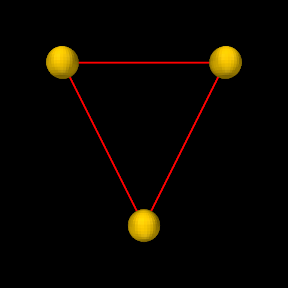
\includegraphics[]{images/RenderSpheresLines}
 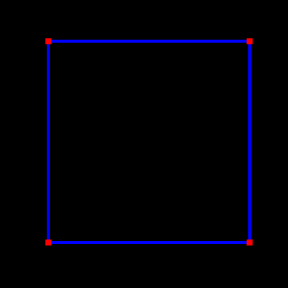
\includegraphics[]{images/RenderSquare}
\else
 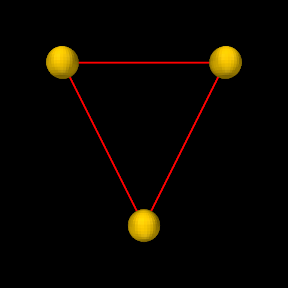
\includegraphics[width=2.5in]{images/RenderSpheresLines}
 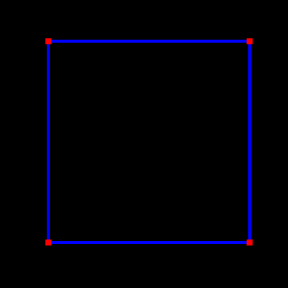
\includegraphics[width=2.5in]{images/RenderSquare}
\fi
\end{tabular}
\end{center}
\caption{Rendered images produced with sample implementations of {\tt render()}.}
\label{renderExamples:fig}
\end{figure}

A {\tt Renderer} also contains {\it draw mode} methods to implement the drawing of points,
lines and triangles in a manner similar to the {\it immediate mode} of legacy OpenGL,
%
\begin{lstlisting}[]
   renderer.beginDraw (drawModeType);

      ... define vertices and normals ...

   renderer.endDraw();
\end{lstlisting}
%
where {\tt drawMode} is an instance
of \javaclass[maspack.render]{Renderer\$DrawMode} and includes points,
lines, line strips and loops, triangles, and triangle strips and
fans. The draw mode methods include:
%
\begin{methodtable}{0.48}{0.52}
\midline
%
\methodentry
{maspack.render.Renderer.beginDraw(DrawMode)}%
{void beginDraw(DrawMode mode)}%
{Begin a draw mode sequence.}%
%
\methodentry
{maspack.render.Renderer.addVertex(Vector3d)}%
{void addVertex(Vector3d vtx)}%
{Add a vertex to the object being drawn.}%
%
\methodentry
{maspack.render.Renderer.setNormal(Vector3d)}%
{void setNormal(Vector3d nrm)}%
{Sets the current vertex normal for the object being drawn.}%
%
\methodentry
{maspack.render.Renderer.endDraw()}%
{void endDraw()}%
{Finish a draw mode sequence.}%
%
\midline
\end{methodtable}
%
The {\tt render()} implementation below uses draw mode to
render the image shown in Figure \ref{renderExamples:fig}, right:
%
\begin{lstlisting}[]
public void render (Renderer renderer, int flags) {
   // the corners of the square
   Vector3d p0 = new Vector3d (0, 0, 0);
   Vector3d p1 = new Vector3d (1, 0, 0);
   Vector3d p2 = new Vector3d (1, 0, 1);
   Vector3d p3 = new Vector3d (0, 0, 1);
   
   renderer.setShading (Shading.NONE);  // turn off lighting

   renderer.setPointSize (6);

   renderer.beginDraw (DrawMode.POINTS);
   renderer.setColor (Color.RED);
   renderer.addVertex (p0);
   renderer.addVertex (p1);
   renderer.addVertex (p2);
   renderer.addVertex (p3);
   renderer.endDraw();

   renderer.setLineWidth (3);
   renderer.setColor (Color.BLUE);
   renderer.beginDraw (DrawMode.LINE_LOOP);
   renderer.addVertex (p0);
   renderer.addVertex (p1);
   renderer.addVertex (p2);
   renderer.addVertex (p3);
   renderer.endDraw();

   renderer.setShading (Shading.FLAT);  // restore lighting  // sphere centers
}
\end{lstlisting}
%
Finally, a {\tt Renderer} contains methods for the rendering of {\it
render objects}, which are collections of vertex, normal and color
information that can be rendered quickly; it may be more efficient to
use render objects for complex rendering involving large numbers of
primitives. Full details on this, and other features of the rendering
interface, are given in the ``Rendering'' section of the
\artisynthManual{maspack}{Maspack Reference Manual}.

\subsection{Implementing custom rendering}

There are two easy ways to add custom rendering to a model:

\begin{enumerate}

\item Override the root model's {\tt render()} method;

\item Define a custom rendering component, with its own {\tt render()} method, and add it to
the model. This approach is more modular and makes it easier to reuse
the rendering between models.

\end{enumerate}

To override the root model render method, one simply adds the
following declaration to the model's definition:
%
\begin{lstlisting}[]
   void render (Renderer renderer, int flags) {
      super.render (renderer, flags);
      
      ... custom rendering code goes here ...

   }
\end{lstlisting}
%
A call to {\tt super.render()} is recommended to ensure that any
rendering done by the model's base class will still occur. Subsequent
statements should then use the {\tt renderer} object to perform
whatever rendering is required, using methods such as described in
Section \ref{RenderMethods:sec} or in the ``Rendering'' section of the
\artisynthManual{maspack}{Maspack Reference Manual}.

To create a custom rendering component, one can simply declare a subclass
of \javaclass[artisynth.core.modelbase]{RenderableComponentBase}
with a custom {\tt render()} method:
%
\begin{lstlisting}[]
import artisynth.core.modelbase.*;
import maspack.render.*;

class MyRenderComp extends RenderableComponentBase {
  
   void render (Renderer renderer, int flags) {
      
      ... custom rendering code goes here ...

   }
}
\end{lstlisting}
%
There is no need to call {\tt super.render()} since 
\javaclass[artisynth.core.modelbase]{RenderableComponentBase} 
does not provide an implementation of {\tt render()}.  It does,
however, provide default implementations of everything else required
by the \javaclass[maspack.render]{Renderable} interface. This includes
exporting render properties via the composite property {\sf
renderProps}, which the {\tt render()} method may use to control the
rendering appearance in a manner consistent with
Section \ref{SettingRenderProperties:sec}. It also includes an
implementation of {\tt prerender()} which by default does nothing.  As
discussed more in Section \ref{PrerenderMethod:sec}, this is often
acceptable {\it unless}:

\begin{enumerate}

\item rendering will be adversely affected by quantities
being updated asynchronously within the simulation;

\item the component contains subcomponents that also need to be rendered.

\end{enumerate}

Once a custom rendering component has been defined, it can be created
and added to the model within the {\tt build()} method:
%
\begin{lstlisting}[]
   MechModel mech; 
   ...

   MyRenderComp rcomp = new MyRenderComp();
   mech.addRenderable (rcomp);
\end{lstlisting}
%
In this example, the component is added to the {\tt MechModel}'s
subcomponent list {\tt renderables}, which ensures that it will be
found by the rendering code. Methods for managing this list include:
%
\begin{methodtable}{0.55}{0.45}
\midline
%
\methodentry
{\mech.MechModel.addRenderable()}
{void addRenderable(Renderable r)}%
{Adds a renderable to the model.}%
%
\methodentry
{\mech.MechModel.removeRenderable()}
{boolean removeRenderable(Renderable r)}%
{Removes a renderable from the model.}%
%
\methodentry
{\mech.MechModel.clearRenderables()}
{void clearRenderables()}%
{Removes all renderables from the model.}%
%
\methodentry
{\mech.MechModel.renderables()}
{ComponentListView<RenderableComponent> renderables()}%
{Returns the list of all renderables.}%
\midline
\end{methodtable}
%

\subsection{Example: rendering body forces}
\label{RenderingBodyForces:sec}

\begin{figure}[ht]
\begin{center}
\iflatexml
 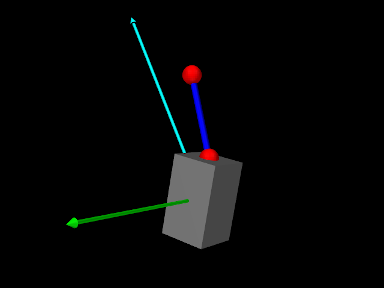
\includegraphics[]{images/BodyForceRendering}
\else
 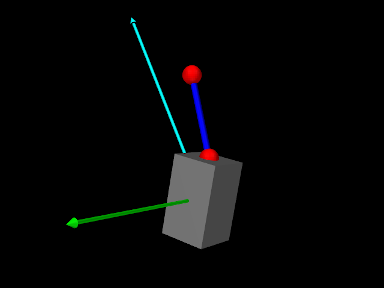
\includegraphics[width=3.75in]{images/BodyForceRendering}
\fi
\end{center}
\caption{{\tt BodyForceRendering} being run in ArtiSynth.}
\label{BodyForceRendering:fig}
\end{figure}

The application model
%
\begin{verbatim}
  artisynth.demos.tutorial.BodyForceRendering
\end{verbatim}
%
gives an example of custom rendering to draw the force and moment
vectors acting on a rigid body as cyan and green arrows,
respectively. The model extends {\tt RigidBodySpring}
(Section \ref{RigidBodySpringExample:sec}), defines a custom
renderable class named {\tt ForceRenderer}, and then uses this to
render the forces on the box in the original model. The code, with the
include files omitted, is listed below:
%
\lstset{numbers=left}
\iflatexml
%% Hack: latexml lstinputlisting doesn't handle firstline correctly
\lstset{firstnumber={-10}}
\lstinputlisting[firstline=1]{../../src/artisynth/demos/tutorial/BodyForceRendering.java}
\lstset{firstnumber={1}}
\else
\lstinputlisting[firstline=12]{../../src/artisynth/demos/tutorial/BodyForceRendering.java}
\fi
\lstset{numbers=none}
%
The force renderer is defined at lines (4-34). For attributes, it
contains a reference to the rigid body, plus scale factors for
rendering the force and moment. Within the {\tt render()} method
(lines 16-33), the force and moment vectors are draw as cyan and green
arrows, starting at the current body position, and scaled by their
respective factors. This scaling is needed to ensure the arrows have a
size appropriate to the viewer, and separate scale factors are needed
because the force and moment vectors have different units. The arrow
radii are given by the renderer's {\sf lineRadius} render property
(lines 22 and 30).

The {\tt build()} method starts by calling the super class {\tt
build()} method to create the original model (line 36), and then uses
{\tt findComponent()} to retrieve its {\tt MechModel}, within which
the ``{\tt box}'' rigid body is located (lines 40-41). A {\tt
ForceRenderer} is then created for this body, with force and moment
scale factors of 0.1 and 0.5, and added to the {\tt MechModel} (lines
44-45). The renderer's {\sf lineRadius} render property is then set to
0.01 (line 48).

To run this example in ArtiSynth, select {\sf All demos > tutorial >
BodyForceRenderer} from the {\sf Models} menu. When run, the model
should appear as in Figure \ref{BodyForceRendering:fig}, showing the
force and moment vectors acting on the box.

\subsection{The {\tt prerender()} method}
\label{PrerenderMethod:sec}

Component {\tt render()} methods are called within ArtiSynth's
graphics thread, and so are called asynchronously with respect to the
simulation thread(s). This means that the simulation may be updating
component attributes, such as positions or forces, at the same time
they are being accessed within {\tt render()}, leading to inconsistent
results in the viewer. While these inconsistencies may not be
significant, particularly if the attributes are changing slowly
between time steps, some applications may wish to avoid them.  For
this, renderable components also implement a
\javamethod[maspack.render.IsRenderable]{prerender()}
method, with the signature
%
\begin{lstlisting}[]
  void prerender (RenderList list);
\end{lstlisting}
%
that is called in synchronization with the simulation prior to
rendering. Its purpose is to:

\begin{itemize}

\item Make copies of simulation-varying attributes so that
they can be used without conflict in the {\tt render()} method;

\item Identify to the system any additional subcomponents that also need
to be rendered.

\end{itemize}

The first task is usually accomplished by copying simulation-varying
attributes into cache variables stored within the component itself.
For example, if a component is responsible for rendering the forces of
a rigid body (as per Section \ref{RenderingBodyForces:sec}), it may
wish to make a local copy of these forces within prerender:
%
\begin{lstlisting}[]
   
   RigidBody myBody;                     // body whose forces are being rendered
   Wrench myRenderForce = new Wrench();  // copy of forces used for rendering

   void prerender (RenderList list) {
      myRenderForce.set (myBody.getForce());
   }

   void render (Renderer renderer, int flags) {
      // do rendering with myRenderForce
      ...
   }
\end{lstlisting}
%

The second task, identifying renderable subcomponents,
is accomplished using the
\javamethod[maspack.render.RenderList]{addIfVisible()}
and 
\javamethod[maspack.render.RenderList]{addIfVisibleAll()}
methods of the
\javaclass[maspack.render]{RenderList} argument, as
in the following examples:
%
\begin{lstlisting}[]
  // additional sub components that need to be rendered
  RenderableComponent mySubCompA;
  RenderableComponent mySubCompB;
 
  void prerender (RenderList list) {
     list.addIfVisible (mySubCompA);
     list.addIfVisible (mySubCompB);
     ...

   }
\end{lstlisting}
%
\begin{lstlisting}[]
  // list of child frame components that also need to be rendered
  RenderableComponentList<Frame> myFrames;

  void prerender (RenderList list) {
     list.addIfVisibleAll (myFrames);
     ...

   }
\end{lstlisting}
%

It should be noted that some ArtiSynth components already support
cached copies of attributes that can be used for rendering.
In particular,
\javaclass[artisynth.core.mechmodels]{Point} (whose
subclasses include {\tt Particle} and {\tt FemNode3d}) uses {\tt
prerender()} to cache its position as an array of {\tt float[]}
which can be obtained using
\javamethod[artisynth.core.mechmodels.Point]{getRenderCoords()},
and 
\javaclass[artisynth.core.mechmodels]{Frame} (whose
subclasses include {\tt RigidBody}) caches its pose as a {\tt
RigidTransform3d} that can be obtained with
\javamethod[artisynth.core.mechmodels.Frame]{getRenderFrame()}.

\section{Point-to-point muscles, tendons and ligaments}
\label{PointToPointMuscles:sec}

Point-to-point muscles are a simple type of component in biomechanical
models that provide muscle-activated forces acting along a line
between two points. ArtiSynth provides this through
\javaclass[artisynth.core.mechmodels]{Muscle}, which is a subclass of
\javaclass[artisynth.core.mechmodels]{AxialSpring} that generates an
active muscle force in response to its {\tt excitation} property. The
excitation property can be set and queried using the methods
% method table
\begin{lstlisting}[]
   setExcitation (double excitation)
   double getExcitation()
\end{lstlisting}
%

As with {\tt AxialSpring}s, {\tt Muscle} components use subclasses of
\javaclass[artisynth.core.materials]{AxialMaterial} to compute the
applied force $f (l, \dot l, a)$ in response to the muscle's length
$l$, length velocity $\dot l$, and excitation signal $a$, which is
assumed to lie in the interval $a \in [0,1]$. Special {\it muscle}
subclasses of {\tt AxialMaterial} exist that compute forces that vary
in response to the excitation. As with other axial materials, this is
done by the material's {\tt computeF()} method, first described in
Section \ref{CustomAxialMaterials:sec}:
%
\begin{lstlisting}[]
  double computeF (l, ldot, l0, excitation)
\end{lstlisting}
%
Usually the force is the sum of a {\it passive} component plus an {\it
active} component that arises in response to the excitation signal.

Once a muscle material is created, it can be assigned to a muscle
or queried using {\tt Muscle} methods
% method table
\begin{lstlisting}[]
  setMaterial (AxialMaterial mat)
  AxialMaterial getMaterial()
\end{lstlisting}
%

\begin{sideblock}
Muscle materials can also be assigned to axial springs, although the
resulting force will always be computed with 0 excitation.
\end{sideblock}

\subsection{Simple muscle materials}
\label{sec:mechii:musclematerials}

A number of simple muscle materials are described below. All compute
force as a function of $a$ and $l$, with an optional damping force
that is proportional to $\dot l$. More complex Hill-type muscles, with
force velocity curves, pennation angle, and a tendon component in
series, are also available and described in
Section \ref{equilibriumMuscles:sec}.

\begin{sideblock}
For historical reasons, the materials {\tt ConstantAxialMuscle}, {\tt
LinearAxialMuscle} and {\tt PeckAxialMuscle}, described below, contain
a property called {\sf forceScaling} that uniformly scales the
computed force. This property is now deprecated, and should therefore
have a value of 1. However, creating these materials with constructors
{\it not} indicated in the documentation below will cause {\sf
forceScaling} to be set to a default value of 1000, thus requiring
that the maximum force and damping values be correspondingly reduced.
\end{sideblock}

\subsubsection{SimpleAxialMuscle}
\label{SimpleAxialMuscle:sec}

\javaclass[artisynth.core.materials]{SimpleAxialMuscle} is the default
{\tt AxialMaterial} for {\tt Muscle}, and is essentially an activated
version of \javaclass[artisynth.core.materials]{LinearAxialMaterial}.
It computes a simple force according to
%
\begin{equation}
f(l, \dot l) = k (l-l_0) + d \dot l + f_{max} \, a,
\label{SimpleAxialMuscle:eqn}
\end{equation}
%
where $l_0$ is the muscle rest length, $k$ and $d$ are stiffness and
damping terms, and $f_{max}$ is the maximum excitation force. $l_0$ is
specified by the {\sf restLength} property of the muscle component,
$a$ by the {\sf excitation} property of the {\tt Muscle}, and $k$, $d$
and $f_{max}$ by the following properties of {\tt
SimpleAxialMuscle}:

\begin{center}
\begin{tabular}{|l|l|l|c|} 
\hline
 & Property & Description & Default \\
\hline
$k$ & {\sf stiffness} & stiffness term & 0 \\
$d$ & {\sf damping} & damping term & 0 \\
$f_{max}$ & {\sf maxForce} & maximum activation force that can be 
imparted by $a$ & 1 \\
\hline
\end{tabular}
\end{center}

{\tt SimpleAxialMuscle}s can be created with the following
constructors:
% method table
\begin{lstlisting}[]
SimpleAxialMuscle()
SimpleAxialMuscle (stiffness, damping, fmax)
\end{lstlisting}
%
where {\tt stiffness}, {\tt damping}, and {\tt fmax} specify $k$, $d$
and $f_{max}$, and properties are otherwise set to their defaults.

\subsubsection{ConstantAxialMuscle}

\javaclass[artisynth.core.materials]{ConstantAxialMuscle}
is a simple muscle material that has a contractile force proportional
to its activation, a constant passive tension, and linear damping.
The resulting force is described by:
%
\begin{equation}
f(\dot l) = f_{max} ( a  +  f_{p} ) + d \dot l.
\label{ConstantAxialMaterial:eqn}
\end{equation}
%
The parameters $f_{max}$, $f_{p}$ and $d$ are specified as properties of
{\tt ConstantAxialMuscle}:

\begin{center}
\begin{tabular}{|l|l|l|c|} \hline
 & Property & Description & Default \\
\hline
$f_{max}$ & {\sf maxForce} & maximum contractile force & 1 \\
$f_{p}$ & {\sf passiveFraction} & 
proportion of $f_{max}$ to apply as passive tension & 0 \\
$d$ & {\sf damping} & damping parameter & 0 \\
\hline
\end{tabular}
\end{center}

{\tt ConstantAxialMuscle}s can be created with the following factory
methods and constructors:
% method table
\begin{lstlisting}[]
ConstantAxialMuscle.create()
ConstantAxialMuscle.create (fmax)
ConstantAxialMuscle (fmax, pfrac)
ConstantAxialMuscle (fmax, pfrac, damping)
\end{lstlisting}
%
where {\tt fmax}, {\tt pfrac}, and {\tt damping} specify $f_{max}$, $f_p$
and $d$, and properties are otherwise set to their defaults.

\begin{sideblock}
Creating a {\tt ConstantAxialMuscle} with the no-args constructor, or
another constructor {\it not} listed above, will cause its {\sf
forceScaling} property (Section \ref{sec:mechii:musclematerials}) to
be set to 1000 instead of 1, thus requiring that {\tt fmax} and {\tt
damping} be corresponding reduced.
\end{sideblock}

\subsubsection{LinearAxialMuscle}

\javaclass[artisynth.core.materials]{LinearAxialMuscle}
is a simple muscle material that has a linear relationship between
length and tension, as well as linear damping. Given a normalized
length described by
%
\begin{equation}
\hat l= \frac{l - l_{opt}}{l_{max} - l_{opt}}, 
\quad \mathrm{with}~ 0 \le \hat l \le 1~\mathrm{enforced},
\end{equation}
%
the force generated by this material is:
%
\begin{equation}
f(l, \dot l) = f_{max} \left( a \hat l +  f_{p} \hat l \, \right) + d \dot l.
\label{LinearAxialMaterial:eqn}
\end{equation}
%
The parameters are specified as properties of {\tt LinearAxialMaterial}:

\begin{center}
\begin{tabular}{|l|l|l|c|} \hline
& Property & Description & Default \\
\hline
$f_{max}$ & {\sf maxForce} & maximum contractile force & 1 \\
$f_{p}$ & {\sf passiveFraction} & 
proportion of $f_{max}$ that forms the maximum passive force & 0 \\
$l_{max}$ & {\sf maxLength} &
length beyond which maximum passive and active forces are generated & 1 \\
$l_{opt}$ & {\sf optLength} &
length below which zero active force is generated & 0 \\
$d$ & {\sf damping} & damping parameter & 0 \\
\hline
\end{tabular}
\end{center}

{\tt LinearAxialMuscle}s can be created with the following factory
methods and constructors:
% method table
\begin{lstlisting}[]
LinearAxialMuscle.create()
LinearAxialMuscle.create (fmax, lrest)
LinearAxialMuscle (fmax, lopt, lmax, pfrac)
LinearAxialMuscle (fmax, lopt, lmax, pfrac, damping)
\end{lstlisting}
%
where {\tt fmax}, {\tt lopt}, {\tt lmax}, {\tt pfrac} and {\tt
damping} specify $f_{max}$, $l_{opt}$, $l_{max}$, $f_{p}$ and $d$,
{\tt lrest} specifies $l_{opt}$ and $l_{max}$ via
$l_{opt} = \mathrm{\tt lrest}$ and
$l_{max} = 3/2 \; \mathrm{\tt lrest}$, and other properties are set to
their defaults.

\begin{sideblock}
Creating a {\tt LinearAxialMuscle} with the no-args constructor, or
another constructor {\it not} listed above, will cause its {\sf
forceScaling} property (Section \ref{sec:mechii:musclematerials}) to
be set to 1000 instead of 1, thus requiring that {\tt fmax} and {\tt
damping} be corresponding reduced.
\end{sideblock}

\subsubsection{PeckAxialMuscle}

The \javaclass[artisynth.core.materials]{PeckAxialMuscle}
material generates a force as described in~\cite{peck2000dynamic}. 
It has a typical Hill-type active force-length relationship (modeled
as a cosine), but the passive force-length properties are linear. This
muscle model was empirically verified for jaw muscles during wide jaw
opening.

\begin{figure}[ht]
\begin{center}
\begin{tabular}{cc}
   \iflatexml
      \includegraphics[width=3in]{images/PeckAPFLC}&
      \includegraphics[width=3in]{images/PeckCFLC}
   \else
      \includegraphics[width=3in]{images/PeckAPFLC}&
      \includegraphics[width=3in]{images/PeckCFLC}
   \fi
\end{tabular}
\end{center}
\caption{Left: active (red) and passive force length curve (green)
for a {\tt PeckAxialMuscle} with $f_{max} = 1$, $f_{p} = 1$, $T_r =
0$, $l_{opt} = 1$, $l_{max} = 2$, and $a = 1$. Note that the passive
force curve is linear for $l \in [l_{opt}, l_{max}]$ and saturates for
$l > l_{max}$. Right: combined active and passive force (blue).}
\label{PeckCurves:fig}
\end{figure}

Given a normalized fibre length described by
%
\begin{equation}
\hat l_f = \frac{l - l_{opt} T_r}{l_{opt} (1 - T_r)}, 
\quad \mathrm{with}~ 1/2 \le \hat l \le 3/2~\mathrm{enforced},
\end{equation}
%
and a normalized muscle length 
%
\begin{equation}
\hat l_m = \frac{l - l_{opt}}{l_{max} - l_{opt}}, 
\quad \mathrm{with}~ 0 \le \hat l \le 1~\mathrm{enforced},
\end{equation}
%
the force generated by this material is:
%
\begin{equation}
f(l, \dot l) = 
f_{max} \left( a \frac{1 + \cos(2 \pi \hat l_f)}{2} +  f_{p} \hat l_m \right) + d \dot l.
\label{PeckAxialMuscle:eqn}
\end{equation}
%
The parameters are specified as properties of {\tt PeckAxialMuscle}:

\begin{center}
\begin{tabular}{|l|l|l|c|} \hline
 & Property & Description & Default \\
\hline
$f_{max}$ & {\sf maxForce} & maximum contractile force & 1 \\
$f_{p}$ & {\sf passiveFraction} & 
proportion of $f_{max}$ that forms the maximum passive force & 0 \\
$T_r$ & {\sf tendonRatio} & tendon to fibre length ratio & 0 \\
$l_{max}$ & {\sf maxLength} & 
length at which maximum passive force is generated & 1 \\
$l_{opt}$ & {\sf optLength} & 
length at which maximum active force is generated & 0 \\
$d$ & {\sf damping} & damping parameter & 0 \\ 
\hline
\end{tabular}
\end{center}

Figure \ref{PeckCurves:fig} illustrates the force length relationship
for a {\tt PeckAxialMuscle}. 

{\tt PeckAxialMuscle}s can be created with the following factory
methods:
% method table
\begin{lstlisting}[]
PeckAxialMuscle.create()
PeckAxialMuscle.create (fmax, lopt, lmax, tratio, pfrac)
PeckAxialMuscle.create (fmax, lopt, lmax, tratio, pfrac, damping)
\end{lstlisting}
%
where {\tt fmax}, {\tt lopt}, {\tt lmax}, {\tt tratio}, {\tt pfrac}
and {\tt damping} specify $f_{max}$, $l_{opt}$, $l_{max}$, $T_r$,
$f_{p}$ and $d$, and other properties are set to their defaults.

\begin{sideblock}
Creating a {\tt PeckAxialMuscle} with the no-args constructor, or
another constructor {\it not} listed above, will cause its {\sf
forceScaling} property (Section \ref{sec:mechii:musclematerials}) to
be set to 1000 instead of 1, thus requiring that {\tt fmax} and {\tt
damping} be corresponding reduced.
\end{sideblock}

\subsubsection{BlemkerAxialMuscle}

The \javaclass[artisynth.core.materials]{BlemkerAxialMuscle} material
generates a force as described in~\cite{blemker:2005:muscle}. It is
the axial muscle equivalent to the constitutive equation along the
muscle fiber direction specified in the
\javaclass[artisynth.core.materials]{BlemkerMuscle} FEM material.

\begin{figure}[ht]
\begin{center}
\begin{tabular}{cc}
   \iflatexml
      \includegraphics[width=3in]{images/BlemkerAPFL}&
      \includegraphics[width=3in]{images/BlemkerCFL}
   \else
      \includegraphics[width=3in]{images/BlemkerAPFL}&
      \includegraphics[width=3in]{images/BlemkerCFL}
   \fi
\end{tabular}
\end{center}
\caption{Left: active force curve $f_L(\hat l)$ (red) and 
passive force curve $f_P(\hat l)$ (green) for a {\tt
BlemkerAxialMuscle} with $l_{opt} = 1$, $l_{max} = 1.4$, $P_1 = 0.05$,
and $P_2 = 6.6$. Right: total force length curve (blue) with 
$f_{max} = 1$ and $a = 1$.}
\label{BlemkerCurves:fig}
\end{figure}

The force produced is a combination of active and passive terms,
plus a damping term, given by
%
\begin{equation}
f(l, \dot l) = 
f_{max} \left( a f_L (\hat l) + f_P (\hat l) \right) + d \dot l,
\label{BlemkerAxialMaterial:eqn}
\end{equation}
%
where $f_{max}$ is the maximum force, $\hat l \equiv l/l_{opt}$ is the
normalized muscle length, and
$f_L (\hat l)$ and $f_P(\hat l)$ are the active and passive
force length curves, given by
%
\begin{equation}
f_L (\hat l) = 
\begin{cases}
9 \, (\hat l - 0.4), & \hat l \in [0.4, 0.6] \\
1 - 4 (1 - \hat l), & \hat l \in [0.6, 1.4] \\
9 \, (\hat l - 1.6), & \hat l \in [1.4, 1.6] \\
0, & \mathrm{otherwise}, \\
\end{cases}
\end{equation}
%
and
%
\begin{equation}
f_P (\hat l) = 
\begin{cases}
0, & \hat l < 1 \\
P_1 (e^{P_2 (\hat l-1)}-1), & \hat l \in [l_{opt}, l_{max}/l_{opt}]\\
P_3 \hat l + P_4, & \hat l > l_{max}/l_{opt}. \\
\end{cases}
\label{BlemkerPassive:eqn}
\end{equation}
%
For the passive force length curve, $P_3$ and $P_4$ are computed to
provide linear extrapolation for $\hat l > l_{max}/l_{opt}$. The other
parameters are specified by properties of {\tt BlemkerAxialMuscle}:

\begin{center}
\begin{tabular}{|l|l|l|c|} 
\hline
 & Property & Description & Default\\
\hline
$f_{max}$ & {\sf maxForce} & the maximum contractile force & $3 \times 10^5$ \\
$P_1$ & {\sf expStressCoeff} & exponential stress coefficient & 0.05 \\
$P_2$ & {\sf uncrimpingFactor} & fibre uncrimping factor & 6.6 \\
$l_{max}$ & {\sf maxLength} & 
length at which passive force becomes linear & 1.4 \\
$l_{opt}$ & {\sf optLength} & 
length at which maximum active force is generated & 1 \\
$d$ & {\sf damping} & damping parameter & 0 \\ 
\hline
\end{tabular}
\end{center}

Figure \ref{BlemkerCurves:fig} illustrates the force length relationship
for a {\tt BlemkerAxialMuscle}. 

{\tt BlemkerAxialMuscle}s can be created with the following 
constructors, 
% method table
\begin{lstlisting}[]
BlemkerAxialMuscle()
BlemkerAxialMuscle (lmax, lopt, fmax, ecoef, uncrimp)
\end{lstlisting}
%
where {\tt lmax}, {\tt lopt}, {\tt fmax}, {\tt ecoef}, and {\tt
uncrimp} specify $l_{max}$, $l_{opt}$, $f_{max}$, $P_1$, $P_2$ and
$d$, and properties are otherwise set to their defaults.

\subsection{Example: muscle attached to a rigid body}
\label{SimpleMuscleExample:sec}

\begin{figure}[ht]
\begin{center}
\iflatexml
 \includegraphics[]{images/SimpleMuscle}
\else
 \includegraphics[width=3.75in]{images/SimpleMuscle}
\fi
\end{center}
\caption{SimpleMuscle model loaded into ArtiSynth.}
\label{SimpleMuscle:fig}
\end{figure}

A simple model showing a single muscle connected to a rigid
body is defined in
%
\begin{verbatim}
  artisynth.demos.tutorial.SimpleMuscle
\end{verbatim}
%

This model is identical to {\tt RigidBodySpring} described in Section
\ref{RigidBodySpringExample:sec}, except that the code to create
the spring is replaced with code to create a muscle
with a {\tt SimpleAxialMuscle} material:
%
\begin{lstlisting}[]
      // create the muscle:      
      muscle = new Muscle ("mus", /*restLength=*/0);
      muscle.setPoints (p1, mkr);
      muscle.setMaterial (
         new SimpleAxialMuscle (/*stiffness=*/20, /*damping=*/10, /*fmax=*/10));
\end{lstlisting}
%
Also, so that the muscle renders differently, the rendering style
for lines is set to {\tt SPINDLE} using the convenience method
%
\begin{lstlisting}[]
      RenderProps.setSpindleLines (muscle, 0.02, Color.RED);
\end{lstlisting}
%

To run this example in ArtiSynth, select {\sf All demos > tutorial >
SimpleMuscle} from the {\sf Models} menu. The model should load and
initially appear as in Figure \ref{SimpleMuscle:fig}.  Running the
model (Section \ref{LoadingAndRunning:sec}) will cause the box to fall
and sway under gravity. To see the effect of the {\tt excitation}
property, select the muscle in the viewer and then choose {\sf Edit
properties ...} from the right-click context menu.  This will open an
editing panel that allows the muscle's properties to be adjusted
interactively. Adjusting the {\tt excitation} property using the
adjacent slider will cause the muscle force to vary.

\subsection{Equilibrium muscles}
\label{equilibriumMuscles:sec}

ArtiSynth supplies several muscle materials that simulate a pennated
muscle in series with a tendon. Both the muscle and tendon generate
forces which are functions of their respective lengths $l_m$ and
$l_t$, and because these components are in series, their respective
forces must be equal when the system is in equilibrium. Given an
overall muscle-tendon length $l \equiv l_m + l_t$, ArtiSynth solves
for $l_m$ at each time step to ensure that this equilibrium condition
is met.

\begin{figure}[h]
\begin{center}
 \includegraphics[width=4in]{images/muscleModel}
\end{center}
\caption{Schematic illustration of an pennated muscle in series with a
tendon.}
\label{equilibriumMuscles:fig}
\end{figure}

A general muscle-tendon system is illustrated by Figure
\ref{equilibriumMuscles:fig}, where $l_m$ and $l_t$ are the muscle and
tendon lengths.  These two components generate forces given by
$f_m(l_m, v_m)$ and $f_t(l_t)$, where $v_m \equiv \dot l_m$, and the
fact that these components are in series implies that their forces
must be in equilibrium:
%
\begin{equation}
f_m(l_m, v_m) = f_t(l_t).
\label{equilibrium:eqn}
\end{equation}
%
The muscle force is in turn produced by a {\it fibre force} $f_f$
acting at an {\it pennation angle} $\phi$ with respect to the
principal muscle direction, such that
%
 \begin{equation*}
f_m = \cos(\phi) f_f (l_f, v_f),
\end{equation*}
%
where $l_f$ is the fibre length, which satisfies
$l_m = \cos(\phi) l_f$, and $v_f \equiv \dot l_f$.

The fibre force is usually computed from the normalized fibre length
$\lfn$ and normalized fibre velocity $\vfn$, defined by
%
\begin{equation}
\lfn = \frac{l_f}{l_o}, \quad \vfn = \frac{v_f}{l_o \vmax},
\label{lfn:eqn}
\end{equation}
%
where $l_o$ is the {\it optimal fibre length} and $\vmax$ is the {\it maximum
contraction velocity}. It is composed of three components in parallel,
such that
%
\begin{equation}
f_f (\lfn, \vfn) = F_o \left( a f_L(\lfn) f_V(\vfn) + f_P(\lfn) +
\beta \vfn \right),
\label{ff:eqn}
\end{equation}
%
where $F_o$ is the {\it maximum isometric force},
$a f_L(\lfn) f_V(\vfn)$ is the active force term induced by an
activation level $a$ and modulated by the {\it active force length
curve} $f_L(\lfn)$ and the {\it force velocity curve} $f_V(\vfn)$,
$f_P(\lfn)$ is the {\it passive force length curve}, and $\beta \vfn$
is an optional damping term induced by a {\it fibre damping} parameter
$\beta$.

The tendon force $f_t(\ltn)$ is computed from 
%
\begin{equation*}
f_t(l_t) = F_o f_T (\ltn),
\end{equation*}
%
where $F_o$ is (again) the maximum isometric force, $f_T(\ltn)$ is the
{\it tendon force length curve} and $\ltn$ is the normalized tendon
length, defined by dividing $l_t$ by the {\it tendon slack length}
$T$:
%
\begin{equation*}
\ltn = \frac{l_t}{T}.
\end{equation*}
%

As the muscle moves, it is assumed that the height $H$ from the fibre
origin to the main muscle line of action remains constant.
This height is defined by
%
\begin{equation*}
H = l_o \sin \phi_o,
\end{equation*}
%
where $\phi_o$ is the {\it optimal pennation angle} at the optimal
fibre length when $l_f = l_o$.

\subsection{Equilibrium muscle materials}
\label{EquilibriumMuscleMaterials:sec}

The equilibrium muscle materials supplied by ArtiSynth include
\javaclass[artisynth.core.materials]{Thelen2003AxialMuscle} and
\javaclass[artisynth.core.materials]{Millard2012AxialMuscle}.  These
are all controlled by properties which specify the parameters
presented in Section \ref{equilibriumMuscles:sec}:

\begin{center}
\begin{tabular}{|l|l|l|c|} 
\hline
& Property & Description & Default\\
\hline
$F_{o}$ & {\sf maxIsoForce} & 
maximum isometric force & 1000 \\
$l_o$ & {\sf optFibreLength} & 
optimal fibre length & 0.1 \\
$T$ & {\sf tendonSlackLength} & 
length beyond which tendon exerts force & 0.2 \\
$\phi_o$ & {\sf optPennationAngle} & 
pennation angle at optimal fibre length (radians) & 0 \\
$\vmax$ & {\sf maxContractionVelocity} & 
maximum contraction velocity & 10 \\
$\beta$ & {\sf fibreDamping} & 
damping parameter for normalized fibre velocity & 0 \\
\hline
\end{tabular}
\end{center}

The materials differ from each other with respect to their active,
passive and tendon force length curves ($f_L(\lfn)$, $f_P(\lfn)$, and
$f_T(\ltn)$) and their force velocity curves ($f_V(\vfn)$).

For a given muscle instance, it is typically only necessary to specify
$F_o$, $l_o$, $T$ and $\phi_o$, where $F_o$, $l_o$ and $T$ are given
in the model's basic force and length units. $\vmax$ is given in units
of $l_o$ per second and has a default value of 10; changing this value
will stretch or contract the domain of the force velocity curve
$f_V(\vfn)$. The damping parameter $\beta$ imparts a damping force
proportional to $\vfn$ and has a default value of 0 (i.e., no
damping). It is often not necessary to add fibre damping (since
damping can be readily applied to the model in other ways), but
$\beta$ is supplied for formulations that do specify damping.  If
non-zero, $\beta$ is usually set to a value less than or equal to
$0.1$.

In addition to the above parameters, equilibrium muscle materials also
export the following properties to adjust their behavior:

\begin{center}
\begin{tabular}{|l|l|l|} 
\hline
Property & Description & Default \\
\hline
{\sf rigidTendon} & forces the tendon to be rigid & {\tt false} \\
{\sf ignoreForceVelocity} & 
ignore the force velocity curve $f_V(\vfn)$ & {\tt false} \\
\hline
\end{tabular}
\end{center}

If {\tt rigidTendon} is {\tt true}, the tendon will be assumed to be
rigid with a length given by the tendon slack length parameter $T$.
This simplifies the muscle computations since $l_m$ is then given by
$l_m = l - T$ and there is no need to compute an equilibrium position.
If {\tt ignoreForceVelocity} is {\tt true}, then force velocity
effects are ignored by replacing the force velocity curve $f_V(\vfn)$
with $1$.

The different equilibrium muscle materials are now summarized:

\subsubsection{Millard2012AxialMuscle}
\label{Millard2012AxialMuscle:sec}

\javaclass[artisynth.core.materials]{Millard2012AxialMuscle}
implements the default version of the {\tt
Millard2012EquilibriumMuscle} model supplied by OpenSim
\cite{delp2007opensim} and described in \cite{millard2013flexing}.

The active, passive and tendon force length curves ($f_L(\lfn)$,
$f_P(\lfn)$, and $f_T(\ltn)$) and force velocity curve ($f_V(\vfn)$)
are implemented using cubic Hermite spline curves to conform closely
to the default curve values provided by OpenSim's {\tt
Millard2012EquilibriumMuscle}. Plots of these curves are shown in
Figures \ref{MillardCurvesA:fig} and \ref{MillardCurvesB:fig}.  Both
the passive and tendon force curves are linearly extrapolated (and
hence exhibit constant stiffness) past $\lfn = 1.7$ and
$\ltn = 1.049$, respectively, with stiffness values of 2.857 and
29.06.

\begin{figure}[ht]
\begin{center}
\begin{tabular}{cc}
   \iflatexml
      \includegraphics[width=3in]{images/MillardAFLC}&
      \includegraphics[width=3in]{images/MillardPFLC}
   \else
      \includegraphics[width=3in]{images/MillardAFLC}&
      \includegraphics[width=3in]{images/MillardPFLC}
   \fi
\end{tabular}
\end{center}
\caption{Default active force length curve $f_L(\lfn)$ (left) and 
passive force length curve $f_P(\lfn)$ (right) for the Millard 2012
muscle material.}
\label{MillardCurvesA:fig}
\end{figure}

\begin{figure}[ht]
\begin{center}
\begin{tabular}{cc}
   \iflatexml
      \includegraphics[width=3in]{images/MillardFVC}&
      \includegraphics[width=3in]{images/MillardTFLC}
   \else
      \includegraphics[width=3in]{images/MillardFVC}&
      \includegraphics[width=3in]{images/MillardTFLC}
   \fi
\end{tabular}
\end{center}
\caption{Default force velocity curve $f_V(\vfn)$ (left) 
and tendon force length curve $f_T(\ltn)$ (right) for the Millard 2012
muscle material. Note that the tendon force curve is about 10 times
stiffer than the passive force curve, as seen by that fact the tendon
curve is shown with a horizontal range of $[0.9, 1.1]$ vs. $[0, 2]$
for the passive curve.}
\label{MillardCurvesB:fig}
\end{figure}

\begin{sideblock}
OpenSim requires that the {\tt Millard2012EquilibriumMuscle} always
exhibits a small bias activation, even when the activation should be
zero, in order to avoid a singularity in the computation of the muscle
length. ArtiSynth computes the muscle length in a manner that makes
this unnecessary.
\end{sideblock}

{\tt Millard2012AxialMuscle}s can be created using the constructors
% method table
\begin{lstlisting}[]
Millard2012AxialMuscle()
Millard2012AxialMuscle(fmax, lopt, tslack, optPenAng)
\end{lstlisting}
%
where {\tt fmax}, {\tt lopt}, {\tt tslack}, and {\tt optPenAng}
specify $F_{o}$, $l_o$, $T$, and $\phi_o$, and other properties are
set to their defaults.

\subsubsection{Thelen2003AxialMuscle}
\label{Thelen2003AxialMuscle:sec}

\javaclass[artisynth.core.materials]{Thelen2003AxialMuscle} implements
the {\tt Thelen2003Muscle} model supplied by OpenSim
\cite{delp2007opensim} and introduced in \cite{thelen2003adjustment}.

The active and passive force length curves are described by
%
\begin{equation}
f_L(\lfn) = e^{-(\lfn-1)^2/\gamma}
\end{equation}
%
and
%
\begin{equation}
f_P(\lfn) = \frac{e^{k^{PE} (\lfn-1)/\eps_0^M}-1}{e^{k^{PE}-1}},`
\end{equation}
%
where $\gamma$, $k^{PE}$, and $\eps_0^M$ are parameters, described
in \cite{thelen2003adjustment}, that control the curve shapes.  These
are exposed as properties of {\tt Thelen2003AxialMuscle} and are
described in Table \ref{ThelenProps:tab}.

The tendon force length curve is described by
\begin{equation}
f_T(\ltn) = 
\begin{cases}
0, & \ltn < 1 \\
\dfrac{F_{toe}}{e^{k_{toe}}-1}(e^{k_{toe} (\ltn-1)/\eps^T_{toe}}-1), &
\ltn \le 1+\eps^T_{toe}\\
k_{lin} (\ltn - 1 - \eps^T_{toe}) + F_{toe}, &
\ltn  > 1+\eps^T_{toe},
\end{cases}
\label{Thelen2003TFLC:eqn}
\end{equation}
%
where $F_{toe}$, $k_{toe}$, $k_{lin}$ and $\eps^T_{toe}$ are
parameters, described in \cite{thelen2003adjustment}, that control the
curve shape. The values of these are either fixed, or derived from the
{\it maximum isometric tendon strain} $\eps_0^T$ (controlled by the
{\sf fmaxTendonStrain} property, Table \ref{ThelenProps:tab}),
according to
%
\begin{equation}
F_{toe} = 0.33, \quad k_{toe} = 3.0, \quad
\eps^T_{toe} = \frac{99 \eps_0^T e^3}{166 e^3 - 67}, \quad
k_{lin} = \frac{0.67}{\eps_0^T - \eps^T_{toe}}.
\label{Thelen2003TFLCParams:eqn}
\end{equation}
%

\begin{table}[h]
\begin{center}
\begin{tabular}{|l|l|l|c|} 
\hline
& Property & Description & Default\\
\hline
$\gamma$ & {\sf kShapeActive} & 
shape factor for active force length curve & 0.45 \\
$k^{PE}$ & {\sf kShapePassive} & 
shape factor for active force length curve & 5.0 \\
$\eps_0^M$ & {\sf fmaxMuscleStrain} & 
passive muscle strain at maximum isometric muscle force & 0.6 \\
$\eps_0^T$ & {\sf fmaxTendonStrain} & 
tendon strain at maximum isometric muscle force & 0.04 \\
$A_f$ & {\sf af} & 
force velocity shape factor & 0.25 \\
$\Flen$ & {\sf flen} & 
maximum normalized lengthening force & 1.4 \\
& {\sf fvLinearExtrapThreshold} &
$\vfn$ beyond which $f_V(\vfn)$ is linearly extrapolated & 0.95\\
\hline
\end{tabular}
\end{center}
\caption{Properties of {\tt Thelen2003AxialMuscle} that control
the shapes of the force curves.}
\label{ThelenProps:tab}
\end{table}

The force velocity curve is determined from equation (6)
in \cite{thelen2003adjustment}. In the notation used by that equation
and the accompanying equation (7), $V^M/V^M_\text{max} = \vfn$, $f_l =
f_L(\lfn)$, and $\bar F^M = a f_L(\lfn) f_V(\vfn)$. Inverting equation
(6) yields the force velocity curve:
%
\begin{equation*}
f_v = 
\begin{cases}
\dfrac {\alpha + \bar{v}^M}{\alpha -\bar{v}^M/A_f}, & \bar{v}^M \le 0 \\[1.5em]
\dfrac {\beta + \bar{v}^M \Flen}{\beta + \bar{v}^M},
& \bar{v}^M > 0,
\end{cases}
\label{fv:eqn}
\end{equation*}
%
where
%
\begin{equation*}
\alpha \equiv 0.25 + 0.75 a, \qquad 
\beta \equiv \alpha \frac{\Flen - 1}{2 + 2/A_f},
\end{equation*}
%
and $a$ is the activation level. Parameters include the {\it maximum
normalized lengthening force} $\Flen$, and force velocity shape factor
$A_f$, described in Table \ref{ThelenProps:tab}.

Plots of the curves resulting from the above equations are shown, for
default values, in Figures \ref{ThelenCurvesA:fig}
and \ref{ThelenCurvesB:fig}.

\begin{figure}[ht]
\begin{center}
\begin{tabular}{cc}
   \iflatexml
      \includegraphics[width=3in]{images/ThelenAFLC}&
      \includegraphics[width=3in]{images/ThelenPFLC}
   \else
      \includegraphics[width=3in]{images/ThelenAFLC}&
      \includegraphics[width=3in]{images/ThelenPFLC}
   \fi
\end{tabular}
\end{center}
\caption{Default active force length curve $f_L(\lfn)$ (left) and 
passive force length curve $f_P(\lfn)$ (right) for the Thelen 2003
muscle material. Note that the passive curve is exponential and does
{\it not} transition to a constant slope for high values of $\lfn$.}
\label{ThelenCurvesA:fig}
\end{figure}

\begin{figure}[ht]
\begin{center}
\begin{tabular}{cc}
   \iflatexml
      \includegraphics[width=3in]{images/ThelenFVC}&
      \includegraphics[width=3in]{images/ThelenTFLC}
   \else
      \includegraphics[width=3in]{images/ThelenFVC}&
      \includegraphics[width=3in]{images/ThelenTFLC}
   \fi
\end{tabular}
\end{center}
\caption{Default force velocity curve $f_V(\vfn)$ (left) and tendon
force length curve $f_T(\ltn)$ (right) for the Thelen 2003 muscle
model. Since the force velocity curve also depends on the activation,
its plot shows the curve for two activation values: 1.0 (dark
magenta), and 0.5 (light magenta).}
\label{ThelenCurvesB:fig}
\end{figure}

{\tt Thelen2003AxialMuscle}s can be created using the constructors
% method table
\begin{lstlisting}[]
Thelen2003AxialMuscle()
Thelen2003AxialMuscle(fmax, lopt, tslack, optPenAng)
\end{lstlisting}
%
where {\tt fmax}, {\tt lopt}, {\tt tslack}, and {\tt optPenAng}
specify $F_{o}$, $l_o$, $T$, and $\phi_o$, and other properties are
set to their defaults.

% LATER \section{Mesh components}
%OPTIONAL 
% LATER \subsection{Fixed meshes}
% LATER \subsection{Simple mesh example}

% SimpleMesh

% LATER \subsection{Skinned meshes}
% LATER \subsection{Simple skinned mesh example}

% SimpleSkinnedMesh

\subsection{Tendons and ligaments}
\label{TendonsAndLigaments:sec}

Special point-to-point spring materials are also available to model
tendons and ligaments. Because these are passive materials, they would
normally be assigned to {\tt AxialSpring} instead of {\tt Muscle}
components, although they will also work correctly in the latter.  The
materials include:

\subsubsection{Millard2012AxialTendon}

\javaclass[artisynth.core.materials]{Millard2012AxialTendon}
implements the default tendon material of the {\tt
Millard2012AxialMuscle} (Section \ref{Millard2012AxialMuscle:sec}),
with a force length relationship given by
%
\begin{equation}
f(l) = F_o f_T (\ltn), \quad \ltn \equiv \frac{l}{T},
\end{equation}
%
where $F_o$ is the maximum isometric force, $f_T()$ is the {\it tendon
force length curve} (shown in Figure \ref{MillardCurvesB:fig},
right), and $T$ is the tendon slack length. $F_o$ and $T$ are specified
by the following properties of {\tt Millard2012AxialTendon}:

\begin{center}
\begin{tabular}{|l|l|l|c|} 
\hline
& Property & Description & Default\\
\hline
$F_{o}$ & {\sf maxIsoForce} & 
maximum isometric force & 1000 \\
$T$ & {\sf tendonSlackLength} & 
length beyond which tendon exerts force & 0.2 \\
\hline
\end{tabular}
\end{center}

{\tt Millard2012AxialTendon}s can be created with the constructors
% method table
\begin{lstlisting}[]
Millard2012AxialTendon()
Millard2012AxialTendon (fmax, tslack)
\end{lstlisting}
%
where {\tt fmax} and {\tt tslack} specify $F_{o}$ and $T$, and
other properties are set to their defaults.

\subsubsection{Thelen2003AxialTendon}

\javaclass[artisynth.core.materials]{Thelen2003AxialTendon}
implements the default tendon material of the {\tt
Thelen2003AxialMuscle} (Section \ref{Thelen2003AxialMuscle:sec}),
with a force length relationship given by
%
\begin{equation}
f(l) = F_o f_T (\ltn), \quad \ltn \equiv \frac{l}{T},
\end{equation}
%
where $F_o$ is the maximum isometric force, $f_T()$ is the {\it tendon
force length curve} described by equation (\ref{Thelen2003TFLC:eqn}),
and $T$ is the tendon slack length. $F_o$, $T$, and the {\it maximum
isometric tendon strain} $\eps_0^T$ (used to determine the parameters
of (\ref{Thelen2003TFLC:eqn}), according to (\ref{Thelen2003TFLCParams:eqn})),
are specified by the following properties of {\tt
Thelen2003AxialTendon}:

\begin{center}
\begin{tabular}{|l|l|l|c|} 
\hline
& Property & Description & Default\\
\hline
$F_{o}$ & {\sf maxIsoForce} & 
maximum isometric force & 1000 \\
$T$ & {\sf tendonSlackLength} & 
length beyond which tendon exerts force & 0.2 \\
$\eps_0^T$ & {\sf fmaxTendonStrain} & 
tendon strain at maximum isometric muscle force & 0.04 \\
\hline
\end{tabular}
\end{center}

{\tt Thelen2003AxialTendon}s can be created with the constructors
% method table
\begin{lstlisting}[]
Thelen2003AxialTendon()
Thelen2003AxialTendon (fmax, tslack)
\end{lstlisting}
%
where {\tt fmax} and {\tt tslack} specify $F_{o}$ and $T$, and
other properties are set to their defaults.

\subsubsection{Blankevoort1991AxialLigament}

\javaclass[artisynth.core.materials]{Blankevoort1991AxialLigament}
implements the {\tt Blankevoort1991Ligament} model supplied
by OpenSim \cite{delp2007opensim} and described in
\cite{blankevoort1991ligament,smith2016influence}.

With the ligament strain and its derivative defined by
%
\begin{equation}
\eps \equiv \frac{l-l_0}{l_0}, \quad \dot\eps \equiv \frac{\dot l}{l_0},
\end{equation}
%
the ligament force is given by
%
\begin{equation}
f(l,\dot l) = f_e(\eps) + f_d(\dot \eps),
\end{equation}
%
where
%
\begin{equation*}
f_e(\eps) = 
\begin{cases}
0, & \eps < 0 \\
\dfrac{1}{2 \eps_t} k \eps^2, & 0 \le \eps \le \eps_t\\
k(\eps - \dfrac{\eps_t}{2}), & \eps > \eps_t,
\end{cases}
\end{equation*}
%
and
%
\begin{equation*}
f_d(\dot\eps) = 
\begin{cases}
d \dot\eps,  & \eps > 0 \; \mathrm{and} \; \dot\eps > 0 \\
0, & \mathrm{otherwise}.
\end{cases}
\end{equation*}
%
The parameters $l_0$, $\eps_t$, $k$, and $d$ are specified by the following
properties of {\tt Blankevoort1991Ligament}:

\begin{center}
\begin{tabular}{|l|l|l|c|} 
\hline
& Property & Description & Default\\
\hline
$l_0$ & {\sf slackLength} &
ligament slack length & 0 \\
$\eps_t$ & {\sf transitionStrain} & 
strain at transition from toe to linear & 0.06 \\
$k$ & {\sf linearStiffness} & 
maximum stiffness of force-length curve & 100 \\
$d$ & {\sf damping} & 
damping parameter & 0.003 \\
\hline
\end{tabular}
\end{center}

{\tt Blankevoort1991Ligament}s can be created with the constructors
% method table
\begin{lstlisting}[]
Blankevoort1991Ligament()
Blankevoort1991Ligament (stiffness, slackLen, damping)
\end{lstlisting}
%
where {\tt stiffness}, {\tt slackLen} and {\tt damping} specify $k$,
$l_o$ and $d$, and other properties are set to their defaults.

\subsection{Example: muscles with separate tendons}

An alternate way to model the equilibrium muscles of Section
\ref{equilibriumMuscles:sec} is to use {\tt two} separate
point-to-point muscles, attached in series via a connecting particle
with a small mass (and possibly damping), thus implementing the muscle
and tendon components separately. This approach allows the muscle
equilibrium length to be determined automatically by the physical
response of the connecting particle, in a manner similar to that
employed by OpenSim's {\tt Millard2012AccelerationMuscle} (described
in \cite{millard2012computationally}). For the muscle material, one
can use any of the tendonless materials of Section
\ref{sec:mechii:musclematerials}, {\it or} the materials of Section
\ref{equilibriumMuscles:sec} with the properties {\sf rigidTendon} and
{\sf tendonSlackLength} set to {\tt true} and $0$, respectively, while
the tendon material can be one described in Section
\ref{TendonsAndLigaments:sec} or some other suitable passive material.
The implicit integrators used by ArtiSynth should permit relatively
stable simulation of the arrangement.

While it is usually easier to employ the equilibrium muscle materials
of Section \ref{EquilibriumMuscleMaterials:sec}, especially for models
involving wrapping and/or via points (Chapter
\ref{multipointSpringIntro:sec}) where it may be difficult to handle
the connecting particle correctly, in some situations the separate
muscle/tendon method may offer a more versatile solution. It can also
be used to validate the equilibrium muscles, as illustrated by the
application model defined in
%
\begin{verbatim}
  artisynth.demos.tutorial.EquilibriumMuscleDemo
\end{verbatim}
%
which provides a direct comparison of the methods. It creates two
simple instances of a Millard 2012 muscle, one above the other in the
x-z plane, with the top instance implemented using the separate
muscle/tendon method and the bottom instance implemented using an
equilibrium muscle material (Figure
\ref{EquilibriumMuscleDemo:fig}). The application model uses control
and monitoring components introduced in Chapter
\ref{SimulationControl:sec} to drive the simulation and record its
results: a {\it controller} (Section \ref{ControllersAndMonitors:sec})
is used to uniformly extend the length of both muscles; {\it output
probes} (Section \ref{Probes:sec}) are used to record the resulting
tension forces; and a {\it control panel} (Section
\ref{ControlPanels:sec}) is created to allow the user to interactively
adjust some of the muscle parameters.

\begin{figure}[ht]
\begin{center}
\iflatexml
 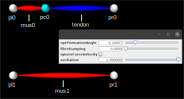
\includegraphics[]{images/EquilibriumMuscleDemo}
\else
 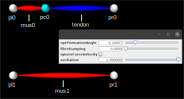
\includegraphics[width=6in]{images/EquilibriumMuscleDemo}
\fi
\end{center}
\caption{{\tt EquilibriumMuscleDemo} loaded into ArtiSynth,
with different particles and muscle components labeled. The separate
muscle/tendon muscle is at the top, the equilibrium muscle at the
bottom, and the control panel is overlaid on the viewer.}
\label{EquilibriumMuscleDemo:fig}
\end{figure}

The code for the {\tt EquilibriumMuscleDemo} class attributes and
{\tt build()} method is shown below:
%
\lstset{numbers=left} 
\iflatexml
%% Hack: latexml lstinputlisting doesn't handle firstline correctly
\lstset{firstnumber={-25}}
\lstinputlisting[firstline=1,lastline=95]{../../src/artisynth/demos/tutorial/EquilibriumMuscleDemo.java}
\lstset{firstnumber={1}}
\else
\lstinputlisting[firstline=27,lastline=121]{../../src/artisynth/demos/tutorial/EquilibriumMuscleDemo.java}
\fi
\lstset{numbers=none}
%
Lines 4-10 declare attributes for muscle parameters and the initial
length of the combined muscle-tendon. Within the {\tt build()} method,
a {\tt MechModel} is created with zero gravity (lines 14-16).  

Next, the separate muscle/tendon muscle is assembled, consisting of
three particles ({\tt pl0}, {\tt pc0}, and {\tt pr0}, lines 20-30), a
muscle {\tt mus0} connected between {\tt pr0} and {\tt pc0} (lines
33-39), and an {\tt tendon} connected between {\tt pc0} and {\tt pr0}
(lines 42-45). Particles {\tt pl0} and {\tt pr0} are both set to be
non-dynamic, since {\tt pl0} will be fixed and {\tt pr0} will be moved
parametrically, while the connecting particle {\tt pc0} has a small
mass and its position is updated by the simulation and so
automatically maintains force equilibrium between the muscle and
tendon. The material {\tt mat0} used for {\tt mus0} is an instance of
{\tt Millard2012AxialMuscle}, with the tendon removed by setting the
{\sf tendonSlackLength} and {\sf rigidTendon} properties to $0$ and
{\tt true}, respectively, while the material for {\tt tendon} is an
instance of {\tt Millard2012AxialTendon}.

The equilibrium muscle is then assembled, consisting of two particles
({\tt pl1} and {\tt pr1}, lines 49-55) and a muscle {\tt mus1}
connected between them (lines 57-61).  {\tt pl1} and {\tt pr1} are
both set to be non-dynamic, since {\tt pl1} will be fixed and {\tt
pr1} will be moved parametrically, and the material {\tt mat1} for
{\tt mus1} is an instance of {\tt Millard2012AxialMuscle} in its
default equilibrium mode. Excitations for both {\tt mus0} and {\tt
mus1} are initialized to 1, and the zero-velocity equilibrium muscle
length is computed using {\tt mat1.computeLmWithConstantVm()} (lines
65-69). This is used to update the muscle position, for {\tt mus0} by
setting the x coordinate of {\tt pc0} and for {\tt mus1} by setting
the internal muscle length variable of {\tt mat1} (lines 71-72).

Render properties for different components are set at lines 76-80, and
then a {\it control panel} is created to allow interactive adjustment
of the muscle material properties {\sf optPennationAngle}, {\sf
fibreDamping}, and {\sf ignoreForceVelocity}, as well the muscle
excitations (lines 83-88). As explained in Sections
\ref{ControlPanelGeneral:sec} and \ref{PropForMultComps:sec}, {\tt
addWidget()} methods are used to create widgets that control each of
these properties for both {\tt mus0} and {\tt mus1}.

At line 92, a {\it controller} is added to the root model to move the
right side particles {\tt p0r} and {\tt p1r} during the simulation,
thus changing the muscles' lengths and hence their tension
forces. Controllers are explained in Section
\ref{ControllersAndMonitors:sec}, and the controller itself is defined
by lines 101-127 of the code listing below. At the start of each
simulation time step, the controller's {\tt apply()} method is called,
with {\tt t0} and {\tt t1} denoting the step's start and end times.
It increases the x positions of {\tt p0r} and {\tt p1r} uniformly with
a speed of {\tt mySpeed} until time {\tt myRunTime/2}, and then
reverses direction until time {\tt myRunTime}. Velocities are also
updated since these are needed to determine $\dot l$ for the muscles'
{\tt computeF()} methods.

Each muscle's tension force is recorded by an {\it output probe}
connected to its {\sf forceNorm} property. Probes are explained in
Section \ref{Probes:sec}; in this example, they are created using the
convenience method {\tt addForceProbe()}, defined by lines 130-140
(below) and called at lines 93-94 in the {\tt build()} method, with
probes for the muscle/tendon and equilibrium muscles named
``muscle/tendon force'' and ``equilibrium force'', respectively.

%
\lstset{numbers=left} 
\iflatexml
%% Hack: latexml lstinputlisting doesn't handle firstline correctly
\lstset{firstnumber={-121}}
\lstinputlisting[firstline=1,lastline=44]{../../src/artisynth/demos/tutorial/EquilibriumMuscleDemo.java}
\lstset{firstnumber={1}}
\else
\lstset{firstnumber={97}}
\lstinputlisting[firstline=123,lastline=166]{../../src/artisynth/demos/tutorial/EquilibriumMuscleDemo.java}
\lstset{firstnumber={1}}
\fi
\lstset{numbers=none}
%

\begin{figure}[ht]
\begin{center}
\begin{tabular}{cc}
\iflatexml
 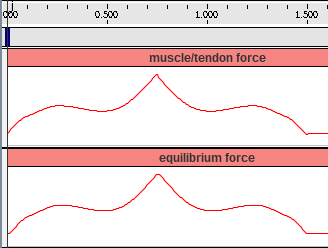
\includegraphics[]{images/EquilibriumMuscleForcesIFV}&
 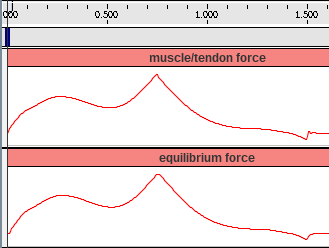
\includegraphics[]{images/EquilibriumMuscleForces}
\else
 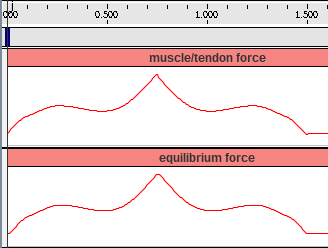
\includegraphics[width=3in]{images/EquilibriumMuscleForcesIFV}&
 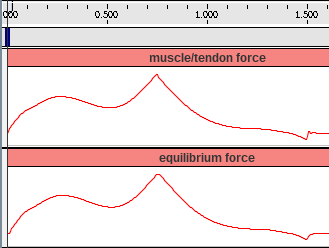
\includegraphics[width=3in]{images/EquilibriumMuscleForces}
\fi
\end{tabular}
\end{center}
\caption{Tension forces produced by {\tt EquilibriumMuscleDemo},
displayed by the output probes, as both muscles are extended and then
contracted. Left and right images show results with the muscle
material property {\sf ignoreForceVelocity} set to {\tt true} and {\tt
false}, respectively.}
\label{EquilibriumMuscleForces:fig}
\end{figure}

To run this example in ArtiSynth, select {\sf All demos > tutorial >
EquilibriumMuscleDemo} from the {\sf Models} menu. The model should
load and initially appear as in Figure
\ref{EquilibriumMuscleDemo:fig}.  As explained above, running the
model will cause the muscles to be extended and contracted by moving
particles {\tt p0r} and {\tt p1r} right and back again. As this
happens, the resulting tension forces can be examined by expanding the
output probes in the timeline (see section ``The Timeline'' in the
\artisynthManual{uiguide}{ArtiSynth User Interface Guide}). The
results are shown in Figure \ref{EquilibriumMuscleForces:fig}, with
the left and right images showing results with the muscle material
property {\sf ignoreForceVelocity} set to {\tt true} and {\tt false},
respectively.

As should be expected, the results for the two muscle implementations
are very similar.  In both cases, the forces exhibit a local peak near
time 0.25 when the muscle lengths are at the maximum of the active
force length curve. As time increases, forces then decrease and then
rise again as the passive force increases, peaking at time 0.75 when
the muscle starts to contract. In the left image, the forces during
contraction are symmetrical with those during extension, while in the
right image the post-peak forces are more attenuated, because in the
latter case the force velocity relationship is enabled as this reduces
forces when a muscle is contracting.

\section{Distance Grids and Components}
\label{DistanceGrids:sec}

Distance grids, implemented by the class
\javaclass[maspack.geometry]{DistanceGrid}, are currently used in
ArtiSynth for both collision handling (Section
\ref{ColliderTypes:sec}) and spring and muscle wrapping around
general surfaces (Section \ref{GeneralSurfaceWrapping:sec}).  A
distance grid is a regular three dimensional grid that is used to
interpolate a scalar distance field and its associated normals.
For collision handling and wrapping purposes, this distance function
is assumed to be signed and is used to estimate the penetration depth
and associated normal direction of a point within some 3D object.

A distance grid consists of $n_x \times n_y \times n_z$ evenly spaced
vertices partitioning a volume into $r_x \times r_y \times r_z$ cuboid
cells, with
%
\begin{equation*}
r_x = n_x-1, \quad r_y = n_y-1, \quad r_z = n_z-1.
\end{equation*}
%
The grid has overall widths $w_x$, $w_y$, $w_z$ along each axis, so
that the widths of each cell are $w_x/r_x$, $w_y/r_y$, $w_z/r_z$. 

Scalar distances and normal vectors are stored at each vertex, and
interpolated at points within each cell using trilinear interpolation.
Distance values (although not normals) can also be interpolated {\it
quadratically} over a composite {\it quadratic} cell composed of $2
\times 2 \times 2$ regular cells. This provides a smoother result than
trilinear interpolation and is currently used for muscle wrapping. To
ensure that all points within the grid can be assigned a unique
quadratic cell, the grid resolution is restricted so that $r_x$,
$r_y$, $r_z$ are always even. Distance grids are typically generated
automatically from mesh data.  More details on the actual
functionality of distance grids is contained in 
the \javaclass[maspack.geometry]{DistanceGrid} API documentation.

When used within ArtiSynth, distance grids are generally contained
within an encapsulating \javaclass[\mech]{DistanceGridComp} component,
which maintains a mesh (or list of meshes) used to generate the grid,
and exports properties for controlling its resolution, mesh fit, and
visualization. For any object that implements
\javaclass[\mech]{CollidableBody} (which includes
\javaclass[\mech]{RigidBody}), its distance grid component can be
obtained using the method
% method table
\begin{lstlisting}
  DistanceGridComp getDistanceGridComp();
\end{lstlisting}
%

A distance grid maintains its own local coordinate system, which is
related to world coordinates by a {\it local-to-world} transform that
can be queried and set via the component methods
\javamethod*[\mech.DistanceGridComp]{setLocalToWorld()} and
\javamethod*[artisynth.core.modelbase.GridCompBase]{getLocalToWorld()}.
For grids associated with a rigid body, the local coordinate system is
synchronized with the rigid body's coordinate system (which
is queried and set via
\javamethod*[\mech.Frame]{setPose()} and
\javamethod*[\mech.Frame]{getPose()}).
The grid's axes are nominally aligned with the local coordinate
system, although they can be subject to an additional orientation
offset (e.g., see the description of the property {\sf fitWithOBB}
below).

By default, a {\tt DistanceGridComp} generates its grid automatically
from its mesh data, within an axis-aligned bounding volume with the
resolutions $r_x$, $r_y$, $r_z$ chosen automatically. However, in
some cases it may be necessary to control the resolution explicitly.
{\tt DistanceGridComp} exports the following properties to control
both the grid's resolution and how it is fit around the mesh data:

\begin{description}

\item[resolution] A vector of 3 integers that specifies the
resolutions $r_x$, $r_y$, $r_z$.  If any value in this vector is set
$\le 0$, then all values are set to zero and
the {\sf maxResolution} property is used to determine the grid
divisions instead.

\item[maxResolution] Sets the default maximum cell resolution that
should be used when constructing the grid. This is the number of cells
that should be used along the {\it longest} bounding volume axis, with the
cell counts along the other axes adjusted to maintain a uniform cell
size. If all three values of {\sf resolution} are $> 0$, those
will be used to specify the cell resolutions instead.

\item[fitWithOBB] If {\tt true}, offsets the orientation of the grid's
x, y, and z axes (with respect to local coordinates) to align with an
oriented bounding box fit to the mesh. Otherwise, the grid axes are
aligned with those of the local coordinate frame.

\item[marginFraction] Specifies the fractional amount by which the
mesh should be extended with respect to a bounding box fit around
the mesh(es). The default value is {\tt 0.1}.

\end{description}

As with all properties, these can be set either interactively (either
using a custom control panel or by selecting the component and then
choosing {\sf Edit properties ...} from the right-click context
menu), or through their set/get accessor methods.  For example, {\sf
resolution} and {\sf maxResolution} can be set and queried via the
methods:
% method table
\begin{lstlisting}[]
   void setResolution (Vector3i res)
   Vector3i getResolution()

   void setMaxResolution (int max)
   int getMaxResolution()
\end{lstlisting}

\begin{figure}[ht]
\begin{center}
  \begin{tabular}{ccc}
    \iflatexml
       \includegraphics[]{images/dumbbellMesh}&
       \includegraphics[]{images/dumbbellDistanceGrid}&
       \includegraphics[]{images/dumbbellDistanceSurface}
    \else
       \includegraphics[width=1.75in]{images/dumbbellMesh}&
       \includegraphics[width=2.5in]{images/dumbbellDistanceGrid}&
       \includegraphics[width=1.75in]{images/dumbbellDistanceSurface}
    \fi
  \end{tabular}
\end{center}
\caption{A mesh used to generate a distance grid, (left), along with a
visualization of the grid itself (middle) and the corresponding
quadratic isosurface (right). Notice how in this case the quadratic
isosurface is smoother than the coarser features of the
original mesh.}
\label{rigidBodySurfacesAndGrid:fig}
\end{figure}

\begin{figure}[ht]
\begin{center}
  \begin{tabular}{cc}
    \iflatexml
       \includegraphics[]{images/dumbbellDistanceGridSub}&
       \includegraphics[]{images/dumbbellDistanceGridGrad}
    \else
       \includegraphics[width=2in]{images/dumbbellDistanceGridSub}&
       \includegraphics[width=2in]{images/dumbbellDistanceGridGrad}
    \fi
  \end{tabular}
\end{center}
\caption{Rendering a subportion of a distance grid
restricted along the x axis by setting {\sf renderRanges} 
to {\tt "9:12 * *"}, with render properties set to show the grid cells
(left), and the vertices and normals (right).}
\label{rigidBodySubGrid:fig}
\end{figure}

When used for either collisions or wrapping, the distance values
interpolated by a distance grid are used to determine whether a point
is inside or outside some 3D object, with the inside/outside boundary
being the isosurface surface corresponding to a distance
value of 0.  This isosurface surface (which differs depending on
whether trilinear or quadratic distance interpolation is used)
therefore represents the effective collision boundary, and it may be
somewhat different from the mesh surface used to generate it. It may
be smoother, or may have discretization artifacts, depending on both
the smoothness and complexity of the mesh and the grid's resolution
(Figure \ref{rigidBodySurfacesAndGrid:fig}).  It is therefore
important to be able to visualize both the trilinear and quadratic
isosurfaces.  {\tt DistanceGridComp} provides a number of properties
to control this along with other aspects of grid visualization:

\begin{description}

\item[renderProps] Render properties that control the colors, styles,
and sizes (or widths) used to render faces, lines and points (Section
\ref{RenderProperties:sec}). Point, line and edge properties are used
for rendering grid vertices, normals, and cell edges, while face
properties are used for rendering the isosurface.
One can select which
components are visible by zeroing appropriate render properties:
zeroing {\tt pointRadius} (or {\tt pointSize}, if the {\tt pointStyle}
is {\tt POINT}) disables drawing of the vertices; zeroing {\tt
lineRadius} (or {\tt lineWidth}, if the {\tt lineStyle} is {\tt LINE})
disables drawing of the normals; and zeroing {\tt edgeWidth}
disables drawing of the cell edges. For an illustration,
see Figure \ref{rigidBodySubGrid:fig}.

\item[renderGrid] If set to {\tt true}, causes the grid's vertices,
normals and cell edges to be rendered, using the render properties as
described above.

\item[renderRanges] Can be used to restrict which part of the distance
grid is drawn. The value is a string which specifies the vertex ranges
along the $x$, $y$, and $z$ axes. In general, the grid will have $n_x
\times n_y \times n_z$ vertices along the $x$, $y$, and $z$ axes,
where $n_x$, $n_y$, and $n_z$ are each one greater than the cell
resolutions $r_x$, $r_y$, and $r_z$. The range string should contain
three range specifications, one for each axis, where each
specification is either {\tt *} (all vertices), {\tt n:m} (vertices in
the index range {\tt n} to {\tt m}, inclusive), or {\tt n} (vertices
only at index {\tt n}). A range specification of {\tt "* * *"} (or
{\tt "*"}) means draw all vertices, which is the default
behavior. Other examples include:
\begin{verbatim}
 "* 7 *"      all vertices along x and z, and those at index 7 along y
 "0 2 3"      a single vertex at indices (0, 2, 3)
 "0:3 4:5 *"  all vertices between 0 and 3 along x, and 4 and 5 along y
\end{verbatim}
For an illustration, see Figure \ref{rigidBodySubGrid:fig}.

\item[renderSurface] If set to {\tt true}, renders the grid's
isosurface, as determined by the {\sf surfaceType} property.
See Figure \ref{rigidBodySurfacesAndGrid:fig}, right.

\item[surfaceType] Controls the interpolation used to form the
isosurface rendered in response to the {\sf renderSurface}
property. {\tt QUADRATIC} (the default) specifies a quadratic
isosurface, while {\tt TRILINEAR} specifies a trilinear isosurface.

\item[surfaceDistance] Controls the level set value used to determine
the isosurface. To render the isosurface used for collision
handling or muscle wrapping, this value should be 0.

\end{description}

When visualizing the isosurface for a distance grid, it is generally
convenient to also turn {\it off} visualization for the meshes used to
generate the grid. For {\tt RigidBody} objects, this can be
accomplished easily using the convenience property {\sf
gridSurfaceRendering}. If set {\tt true}, it will cause the
isosurface to be rendered {\it instead} of its mesh components.  The
isosurface type will be that indicated by the grid component's {\sf
surfaceType} property, and the rendering will occur independently of
the visibility settings for the meshes or the grid component.

\section{Transforming geometry}
\label{TransformingGeometry:sec}

Certain ArtiSynth components, including {\tt MechModel}, implement the
interface \javaclass[artisynth.core.modelbase]{TransformableGeometry},
which allows the geometric transformation of the component's
attributes (such as meshes, points, frame locations, etc.), along with
its descendant components. The interface provides the method
% method table
\begin{lstlisting}[]
   public void transformGeometry (AffineTransform3dBase X);
\end{lstlisting}
%
where {\tt X} is an \javaclass[maspack.matrix]{AffineTransform3dBase}
that may be either a \javaclass[maspack.matrix]{RigidTransform3d} or a
more general \javaclass[maspack.matrix]{AffineTransform3d} (Section
\ref{RigidTransform3d:sec}).

\begin{figure}[ht]
\begin{center}
   \begin{tabular}{ccc}
   \iflatexml
      \includegraphics[width=2truein]{images/tgenModel} &
      \includegraphics[width=2truein]{images/tgenModelRigid} &
      \includegraphics[width=2truein]{images/tgenModelAffine}
   \else
      \includegraphics[width=0.27\textwidth]{images/tgenModel} &
      \includegraphics[width=0.34\textwidth]{images/tgenModelRigid} &
      \includegraphics[width=0.34\textwidth]{images/tgenModelAffine}
   \fi
   \end{tabular}
\end{center}
\caption{Simple illustration of a model (left) undergoing a rigid
transformation (middle) and an affine transformation (right).}
\label{RigidAndAffineTransforms:fig}
\end{figure}

\javamethodAlt{artisynth.core.modelbase.TransformableGeometry.transformGeometry()}%
{transformGeometry(X)}
can be used to translate, rotate, shear or scale components. It
can be applied to an entire model or individual components. Unlike
\javamethod*[artisynth.core.util.ScalableUnits]{scaleDistance()}, it
actually changes the physical geometry and so may change the
simulation behavior. For example, applying {\tt transformGeometry()}
to a \javaclass[artisynth.core.mechmodels]{RigidBody} will cause the
shape of its mesh to change, which will change its mass if its {\sf
inertiaMethod} property is set to {\tt DENSITY}.
Figure \ref{RigidAndAffineTransforms:fig} shows a simplified
illustration of both rigid and affine transformations being applied to
a model.

The example below shows how to apply a transformation to a model in
code. In it, a {\tt MechModel} is first scaled by the factors 1.5, 2,
and 3 along the x, y, and z axes, and then flipped upside down using a
{\tt RigidTransform3d} that rotates it by 180 degrees about the x
axis:
%
\begin{lstlisting}[]
   MechModel mech;

   ... build mech model ...

   AffineTransform3d X = new AffineTransform3d();
   X.applyScaling (1.5, 2, 3);
   mech.transformGeometry (X);
   
   RigidTransform3d T = 
      new RigidTransform3d (/*x,y,z=*/0, 0, 0, /*r,p,y=*/0, 0, Math.PI);
   mech.transformGeometry (T);
\end{lstlisting}
%

\begin{sideblock}
The transform specified to {\tt transformGeometry} is in {\it world}
coordinates. If the component being transformed has its own
local coordinate frame (such as a rigid body), and one wants to
specify the transform in that local frame, then one needs to convert
the transform from local to world coordinates. Let $\T_{CW}$ be the
local coordinate frame, and let $\X_W$ and $\X_B$ be the transform in
world and body coordinates, respectively. Then
%
\begin{equation*}
\X_W \, \T_{CW} = \T_{CW} \, \X_B
\end{equation*}
%
and so
%
\begin{equation*}
\X_W  = \T_{CW} \, \X_B \, \T_{CW}^{-1}.
\end{equation*}
%
(See Appendix \ref{RigidTransforms:sec}
and \ref{AffineTransforms:sec}).  
\end{sideblock}

As an example of converting a transform to world coordinates, suppose
we wish to scale a rigid body by $a$, $b$, and $c$ along its local
axes. The transformation could then be done as follows:
%
\begin{lstlisting}[]
  AffineTransform3d XB = new AffineTransform3d(); // transform in body coords
  AffineTransform3d XW = new AffineTransform3d(); // transform in world coords
  RigidTransform3d TBW = body.getPose(): // coordinate frame of the body

  XB.setScaling (a, b, c);      // set scaling in body coords ...
  XW.mul (TBW, XB);             // ... convert to world coords ...
  XW.mulInverseRight (XW, TBW); 
  body.transformGeometry (XW);  // ... and apply to the body
\end{lstlisting}
%

\subsection{Nonlinear transformations}

The \javaclass[artisynth.core.modelbase]{TransformableGeometry}
interface also supports general, nonlinear geometric transforms.
This can be done using a
\javaclass[maspack.geometry]{GeometryTransformer}, which is an
abstract class for performing general transformations.  To apply such
a transformation to a component, one can create and initialize an appropriate
subclass of {\tt
GeometryTransformer} to perform the desired transformation, and
then apply it using the static {\tt transform} method of the utility class 
\javaclass[artisynth.core.modelbase]{TransformGeometryContext}:
%
\begin{lstlisting}[]
  ModelComponent comp;     // component to be transformed
  GeometryTransformer gtr; // transformer to do the transforming

  ... instantiate and initialize the transformer ...

  TransformGeometryContext.transform (comp, gtr, /*flags=*/0);
\end{lstlisting}
%

At present, the following subclasses of {\tt GeometryTransformer} are
available:

\begin{description}

\item[\protect{\javaclass[maspack.geometry]{RigidTransformer}}]\mbox{}

Implements rigid 3D transformations.

\item[\protect{\javaclass[maspack.geometry]{AffineTransformer}}]\mbox{}

Implements affine 3D transformations.

\item[\protect{\javaclass[artisynth.core.femmodels]{FemGeometryTransformer}}]\mbox{}

Implements a general transformation, using the deformation field
induced by a finite element model. 

\end{description}

\javaclass[artisynth.core.modelbase]{TransformGeometryContext} also
supplies the following convenience methods to apply transformations to
components or collections of components:
% method table
\begin{lstlisting}[]
    void transform (Iterable<TransformableGeometry>, GeometryTransformer, int);
    void transform (TransformableGeometry[], GeometryTransformer, int);

    void transform (TransformableGeometry, AffineTransform3dBase, int);
    void transform (Iterable<TransformableGeometry>, AffineTransform3dBase, int);
    void transform (TransformableGeometry[], AffineTransform3dBase, int);
\end{lstlisting}
%
The last three of these methods create an instance of either
\javaclass[maspack.geometry]{RigidTransformer} or
\javaclass[maspack.geometry]{AffineTransformer} for the supplied
\javaclass[maspack.matrix]{AffineTransform3dBase}. In fact, most
{\tt TransformableGeometry} components implement their
\javamethodAlt{artisynth.core.modelbase.TransformableGeometry.transformGeometry()}%
{transformGeometry(X)} method as follows:
%
\begin{lstlisting}[]
   public void transformGeometry (AffineTransform3dBase X) {
      TransformGeometryContext.transform (this, X, 0);
   }
\end{lstlisting}
%

The \javaclass[artisynth.core.femmodels]{FemGeometryTransformer}
class is derived from the
class \javaclass[maspack.geometry]{DeformationTransformer}, which uses
the single method
\javaclass[maspack.geometry.DeformationTransformer]{getDeformation()} to
obtain deformation field information at a specified reference position:
% method table
\begin{lstlisting}[]
    void getDeformation (Vector3d p, Matrix3d F, Vector3d r)
\end{lstlisting}
%
If the deformation field is described by $\x' = f(\x)$, then
for a given reference position $\r$ (in undeformed coordinates),
this method should return the deformed position $\p = f(\r)$
and the deformation gradient
%
\begin{equation}
\F \equiv \frac{\partial f}{\partial \x}
\end{equation}
%
evaluated at $\r$. 

\javaclass[artisynth.core.femmodels]{FemGeometryTransformer} obtains
$f(\x)$ and $\F$ from a
\javaclass[artisynth.core.femmodels]{FemModel3d} (see Section
\ref{FEMModels:sec}) whose elemental rest positions enclose the
components to be transformed, using the fact that a finite element
model creates an implied piecewise-smooth deformation field as it
deviates from its rest position. For each reference point $\r$ needed
by the transformation process, {\tt FemGeometryTransformer} finds the
FEM element whose rest volume encloses $\r$, and then uses the
corresponding shape function coordinates to compute $f(\x)$ and $\F$
from the element's deformation. If the FEM model does {\it not}
enclose $\r$, the nearest element is used to determine the shape
function coordinates (however, this calculation becomes less accurate and
meaningful the farther $\r$ is from the FEM model). Transformations based
on FEM models are further illustrated in Section
\ref{FemModelDeformer:sec}, and by Figure
\ref{JointedCollideDeformation:fig}. Full details on ArtiSynth finite
element models are given in Section \ref{FEMModels:sec}.

Besides FEM models, there are numerous other ways to create
deformation fields, such as radial basis functions, thin plate
splines, etc. Some of these may be more appropriate for a particular
application and can provide deformations that are globally smooth (as
opposed to piecewise smooth).  It should be relatively easy for an
application to create its own subclass of {\tt DeformationTransformer}
to implement the deformation of choice by overriding the single
\javaclass[maspack.geometry.DeformationTransformer]{getDeformation()}
method.

\subsection{Example: the FemModelDeformer class}
\label{FemModelDeformer:sec}

An FEM-based geometric transformation of a {\tt MechModel} is
facilitated by the class
\javaclass[artisynth.core.workspace]{FemModelDeformer}, which one can
add to an existing {\tt RootModel} to transform the geometry of a {\tt
MechModel} already located within that {\tt RootModel}.  {\tt
FemModelDeformer} subclasses
\javaclass[artisynth.core.femmodels]{FemModel3d} to include a
\javaclass[artisynth.core.femmodels]{FemGeometryTransformer}, and
provides some utility methods to support the transformation process.

A {\tt FemModelDeformer} can be added to a {\tt RootModel} by adding
the following code fragment to the end of the {\tt build()} method:
%
\begin{lstlisting}[]
   public void build (String[] args) {

      ... build the model ...

      FemModelDeformer deformer =
         new FemModelDeformer ("deformer", this, /*maxn=*/10);
      addModel (deformer);
      // add a control panel (this is optional)
      addControlPanel (deformer.createControlPanel());  
   }
\end{lstlisting}
%
When the deformer is created, its constructor searches the specified
{\tt RootModel} to locate the first top-level {\tt MechModel}. It then
creates a hexahedral FEM grid around this model, with {\tt maxn} specifying
the number of cells along the maximum dimension. Material and
mass properties of the model are computed automatically from the
underlying {\tt MechModel} dimensions (but can be altered if necessary after
construction). When added to the {\tt RootModel},
the deformer becomes another top-level model that can be deformed
independently of the {\tt MechModel} to create the required
deformation field, as described below. It also supplies application-defined
menu items that appear under the {\sf Application} menu in the ArtiSynth
menu bar (see Section \ref{MenuItems:sec}). 
The deformer's {\tt createControlPanel()} can also be used
to create a {\tt ControlPanel} (Section \ref{ControlPanels:sec}) that
controls the visibility of the FEM model and the dynamic behavior of
both it and the {\tt MechModel}.

An example is defined in 
%
\begin{verbatim}
  artisynth.demos.tutorial.DeformedJointedCollide
\end{verbatim}
%
where the {\tt JointedCollide} example of Section
\ref{JointedCollide:sec} is extended to include a 
{\tt FemModelDeformer} using the code described above.

\begin{figure}[ht]
\begin{center}
\iflatexml
 \includegraphics[]{images/DeformedJointedCollide}
\else
 \includegraphics[width=5in]{images/DeformedJointedCollide}
\fi
\end{center}
\caption{The {\tt DeformedJointedCollide} example initially loaded
into ArtiSynth.}
\label{DeformedJointedCollide:fig}
\end{figure}

To load this example in ArtiSynth, select {\sf All demos > tutorial >
DeformedJointedCollide} from the {\sf Models} menu. The model should load and
initially appear as in Figure \ref{DeformedJointedCollide:fig}, where
the control panel appears on the right.

The underlying {\tt MechModel} (or "model") can now be
transformed by first deforming the FEM model (or "grid") and
then using the resulting deformation field to effect the
transformation:

\begin{enumerate}

\item Make the model non-dynamic and the grid dynamic by unchecking
{\sf model dynamic} and checking {\sf grid dynamic} in the control
panel. This means that when simulation is run, the model will be inert
while the grid will respond physically.

\item Deform the grid using simulation. One easy way to do this is to
fix certain nodes, generally on or near the grid boundary, and then
move some of these using the translation or transrotator
tool while simulation is running. To fix a set of nodes, select
them in the viewer, choose {\sf Edit properties ...} from the
right-click context menu, and then uncheck their {\sf dynamic} property.
To easily select a large number of nodes without also selecting
model components or grid elements, one can specify {\tt FemNode}
in the selection filter widget. (See the sections
``Transformer Tools'' and ``Selection filtering'' in the
\artisynthManual{uiguide}{ArtiSynth User Interface Guide}.)

\item After the grid has been deformed, choose {\sf deform} from the
{\sf Application} menu in the ArtiSynth toolbar to transform the model.
Afterwards, the transformation can be undone by choosing {\sf undo},
and the grid can be reset by choosing {\sf reset grid}.

\item To run the deformed model after the transformation, it should
again be made dynamic by checking {\sf model dynamic} in the control
panel.  The itself grid can be made non-dynamic, and it and/or its
nodes can be made invisible by unchecking {\sf grid visible} and/or
{\sf grid nodes visible} in the control panel.

\end{enumerate}

The result of a possible deformation is shown in Figure
\ref{JointedCollideDeformation:fig}.

\begin{figure}[ht]
\begin{center}
  \begin{tabular}{cc}
  \iflatexml
    \includegraphics[]{images/DeformedJointedCollideBefore}&
    \includegraphics[]{images/DeformedJointedCollideAfter}
  \else
    \includegraphics[width=0.45\textwidth]{images/DeformedJointedCollideBefore}&
    \includegraphics[width=0.45\textwidth]{images/DeformedJointedCollideAfter}
  \fi
  \end{tabular}
\end{center}
\caption{Deformation achieved in {\tt DeformedJointedCollide},
showing both the model and grid (using an orthographic view)
before and after the deformation.}
\label{JointedCollideDeformation:fig}
\end{figure}

\begin{sideblock}
Note: {\tt FemModelDeformer} is not intended to provide a general
purpose solution to nonlinear geometric transformations. Rather, it
is mainly intended to illustrate the capabilities of
\javaclass[maspack.geometry]{GeometryTransformer} and the
\javaclass[artisynth.core.modelbase]{TransformableGeometry} interface.
\end{sideblock}

\subsection{Implementation and behavior}

As indicated above, the management of transforming the geometry for one
or more components is handled by the
\javaclass[artisynth.core.modelbase]{TransformGeometryContext} class.
The transform operations themselves are carried out by this class's
\javamethod[artisynth.core.modelbase.TransformGeometryContext]{apply()} 
method, which (a) assembles all the components that need
to be transformed, (b) performs the actual transform operations,
(c) invokes any required updating actions on other components,
and finally (d) notifies parent components of the change using
a \javaclass[artisynth.core.modelbase]{GeometryChangeEvent}.

To support this, ArtiSynth components which implement
\javaclass[artisynth.core.modelbase]{TransformableGeometry}
must also supply the methods
% method table
\begin{lstlisting}[]
   public void addTransformableDependencies (
      TransformGeometryContext context, int flags);

   public void transformGeometry (
      GeometryTransformer gtr, TransformGeometryContext context, int flags);
\end{lstlisting}
%
The first method,
\javamethodAlt{%
artisynth.core.modelbase.TransformableGeometry.addTransformableDependencies()}%
{addTransformableDependencies(context,flags)}, 
is called in step (a) to add to the context any additional components
which should be transformed along with this component. This includes
any descendants which should be transformed, since the
transformation of these should not generally be done within\pdfbreak
{\tt transformGeometry(gtr,context,flags)}.

The second method, 
\javamethodAlt{%
artisynth.core.modelbase.TransformableGeometry.transformGeometry(,,)}%
{transformGeometry(gtr,context,flags)}, is
called in step (b) to perform the actual transformation on this
component.  It should use the supplied geometry transformer {\tt gtr}
to transform its attributes, as well as {\tt context} to query what
other components are also being transformed and to request
any needed updating actions to be called in step (c).  The {\tt flags} argument
specifies conditions associated with the transformation, which at the
moment may currently include:

\begin{description}

\item[TG\_SIMULATING]\mbox{}

The system is currently simulating, and therefore it may not be
desirable to transform all attributes;

\item[TG\_ARTICULATED]\mbox{}

Rigid body articulation constraints should
be enforced as the transform proceeds.

\end{description}

Full details for all this are given in the documentation for
\javaclass[artisynth.core.modelbase]{TransformGeometryContext}.

The transforming behavior of a component is up to its implementing
method, but the following rules are generally observed:

\begin{enumerate}

\item Transformable descendants are also transformed, by using {\tt
addTransformableDependencies()} to add them to the context as described
above;

\item When the nodes of an FEM model (Section \ref{FEMModels:sec}) are
transformed, the rest positions are also transformed if the system is
not simulating (i.e., if the {\tt TG\_SIMULATING} flag is not set).
This also causes the mass of the adjacent nodes to be recomputed from
the densities of the adjacent elements;

\item When dynamic components are transformed, any attachments and
constraints associated with them are updated appropriately, but only
if the system is not simulating. Non-transforming dynamic components
that are attached to transforming components as slaves are generally
updated so as to follow the transforming components to which they are
attached.

\end{enumerate}

\subsection{Use in model registration}

Transforming model geometry can obviously be used as part of the
process of creating subject-specific biomechanical and anatomical
models. However, registration will generally require more that
geometric transformation, since other properties, such as material
stiffnesses, densities, and maximum forces will generally need to be
adjusted as well. As a specific example, when applying a geometric
transform to a model containing {\tt AxialSprings}, the {\tt
restLength} properties of the springs will be unchanged, whereas the
initial lengths may be, resulting in a different applied forces and
physical behavior.

\section{General component arrangements}

As discussed in Section \ref{MechModel:sec} and elsewhere, a {\tt
MechModel} provides a number of predefined child components for
storing particles, rigid bodies, springs, constraints, and other
components.  However, applications are not required to store their
components in these containers, and may instead create any sort of
component arrangement desired.

For example, suppose that one wishes to create a biomechanical model
of both the right and left human arms, consisting of bones,
point-to-point muscles, and joints. The standard containers supplied
by \javaclass[artisynth.core.mechmodels]{MechModel} would require that
all the components be placed within the following containers:
%
\begin{lstlisting}[]
   rigidBodies          // all bones
   axialSprings         // all point-to-point muscles
   connectors           // all joints
\end{lstlisting}
%
Instead of this, one may wish to set up a more appropriate component
hierarchy, such as
%
\begin{lstlisting}[]
   leftArm              // left-arm components
      bones             //   left bones
      muscles           //   left muscles
      joints            //   left joints
   rightArm             // right-arm components
      bones             //   right bones
      muscles           //   right muscles
      joints            //   right joints
\end{lstlisting}
%
To do this, the application {\tt build()} method can create the
necessary hierarchy and then
populate it with whatever components are desired.  Before simulation
begins (or whenever the model structure is changed), the {\tt
MechModel} will recursively traverse the component hierarchy and
update whatever internal structures are needed to run the
simulation.

\subsection{Container components}

The generic class \javaclass[artisynth.core.modelbase]{ComponentList}
can be used as a container for model components of a specific type.
It can be created using a declaration of the form
%
\begin{lstlisting}[]
   ComponentList<Particle> list = new ComponentList<Type> (Type.class, name);
\end{lstlisting}
%
where {\tt Type} is the class type of the components and {\tt name} is
the name for the container. Once the container is created, it should
be added to the {\tt MechModel} (or another internal container) and 
populated with child components of the specified type.
For example,
\begin{lstlisting}[]
   MechModel mech; 
   ...
   ComponentList<Particle> parts = 
      new ComponentList<Particle> (Particle.class, "parts");
   ComponentList<Frame> frames = 
      new ComponentList<Frame> (Frame.class, "frames");

   // add containers to the mech model
   mech.add (parts); 
   mech.add (frames);
\end{lstlisting}
creates two containers named {\tt "parts"} and {\tt "frames"} for
storing components of type {\tt Particle} and {\tt Frame},
respectively, and adds them to a {\tt MechModel} referenced by {\tt
mech}.

In addition to {\tt ComponentList}, applications may use several
"specialty" container types which are subclasses of {\tt
ComponentList}:

\begin{description}

\item[RenderableComponentList]\mbox{}

A subclass of {\tt ComponentList}, that
has its {\it own} set of render properties which can be inherited by
its children. This can be useful for compartmentalizing render
behavior.  Note that it is {\it not} necessary to store renderable
components in a {\tt RenderableComponentList}; components stored in a
{\tt ComponentList} will be rendered too.

\item[PointList]\mbox{}

A {\tt RenderableComponentList} that is optimized for
rendering points, and also contains its own {\tt pointDamping}
property that can be inherited by its children.

\item[PointSpringList]\mbox{}

A {\tt RenderableComponentList} designed for
storing point-based springs. It contains a {\tt material} property that
specifies a default axial material that can be used by its children.

\item[AxialSpringList]\mbox{}

A {\tt PointSpringList} that is optimized for
rendering two-point axial springs.

\end{description}

If necessary, it is relatively easy to define one's own customized
list by subclassing one of the other list types. One of the main
reasons for doing so, as suggested above, is to supply default
properties to be inherited by the list's descendants.  

A component list which declares {\tt ModelComponent} as its type can
be used to store {\tt any} type of component, including other
component lists. This allows the creation of arbitrary component
hierarchies. Generally either\pdfbreak
{\tt ComponentList<ModelComponent>} or 
{\tt RenderableComponentList<ModelComponent>} are
best suited to implement hierarchical groupings.

\subsection{Example: a net formed from balls and springs}

\begin{figure}[ht]
\begin{center}
\iflatexml
 \includegraphics[]{images/NetDemo}
\else
 \includegraphics[width=3.75in]{images/NetDemo}
\fi
\end{center}
\caption{NetDemo model loaded into ArtiSynth.}
\label{NetDemo:fig}
\end{figure}

A simple example showing an arrangement of balls and springs formed into
a net is defined in
%
\begin{verbatim}
  artisynth.demos.tutorial.NetDemo
\end{verbatim}
%

The {\tt build()} method and some of the supporting definitions for
this example are shown below.
%
\lstset{numbers=left}
\begin{lstlisting}[]
   protected double stiffness = 1000.0;   // spring stiffness
   protected double damping = 10.0;       // spring damping
   protected double maxForce = 5000.0;    // max force with excitation = 1
   protected double mass = 1.0;           // mass of each ball
   protected double widthx = 20.0;        // width of the net along x
   protected double widthy = 20.0;        // width of the net along y
   protected int numx = 8;                // num balls along x
   protected int numy = 8;                // num balls along y

   // custom component containers
   protected MechModel mech;
   protected PointList<Particle> balls;
   protected ComponentList<ModelComponent> springs;   
   protected RenderableComponentList<AxialSpring> greenSprings;
   protected RenderableComponentList<AxialSpring> blueSprings;

   private AxialSpring createSpring (
      PointList<Particle> parts, int idx0, int idx1) {
      // create a "muscle" spring connecting particles indexed by 'idx0' and
      // 'idx1' in the list 'parts'
      Muscle spr = new Muscle (parts.get(idx0), parts.get(idx1));
      spr.setMaterial (new SimpleAxialMuscle (stiffness, damping, maxForce));
      return spr;
   }

   public void build (String[] args) {

      // create MechModel and add to RootModel
      mech = new MechModel ("mech");
      mech.setGravity (0, 0, -980.0);
      mech.setPointDamping (1.0);
      addModel (mech);

      int nump = (numx+1)*(numy+1); // nump = total number of balls

      // create custom containers:
      balls = new PointList<Particle> (Particle.class, "balls");
      springs = new ComponentList<ModelComponent>(ModelComponent.class,"springs");
      greenSprings = new RenderableComponentList<AxialSpring> (
         AxialSpring.class, "greenSprings");
      blueSprings = new RenderableComponentList<AxialSpring> (
         AxialSpring.class, "blueSprings");

      // create balls in a grid pattern and add to the list 'balls'
      for (int i=0; i<=numx; i++) {
         for (int j=0; j<=numy; j++) {
            double x = widthx*(-0.5+i/(double)numx);
            double y = widthy*(-0.5+j/(double)numy);
            Particle p = new Particle (mass, x, y, /*z=*/0);
            balls.add (p);
            // fix balls along the edges parallel to y
            if (i == 0 || i == numx) {
               p.setDynamic (false);
            }
         }
      }

      // connect balls by green springs parallel to y
      for (int i=0; i<=numx; i++) {
         for (int j=0; j<numy; j++) {
            greenSprings.add (
               createSpring (balls, i*(numy+1)+j, i*(numy+1)+j+1));
         }
      }
      // connect balls by blue springs parallel to x
      for (int j=0; j<=numy; j++) {
         for (int i=0; i<numx; i++) {
            blueSprings.add (
               createSpring (balls, i*(numy+1)+j, (i+1)*(numy+1)+j));
         }
      }

      // add containers to the mechModel
      springs.add (greenSprings);
      springs.add (blueSprings);
      mech.add (balls);
      mech.add (springs);

      // set render properties for the components      
      RenderProps.setLineColor (greenSprings, new Color(0f, 0.5f, 0f));
      RenderProps.setLineColor (blueSprings, Color.BLUE);
      RenderProps.setSphericalPoints (mech, widthx/50.0, Color.RED);
      RenderProps.setCylindricalLines (mech, widthx/100.0, Color.BLUE);
   }
\end{lstlisting}
\lstset{numbers=none}
%
The {\tt build()} method begins by creating a {\tt MechModel} in the
usual way (lines 29-30). It then creates a net composed of a set of
balls arranged as a uniform grid in the x-y plane, connected by a set
of green colored springs running parallel to the y axis and a set of
blue colored springs running parallel to the x axis. These are
arranged into a component hierarchy of the form
%
\begin{lstlisting}[]
   balls
   springs
      greenSprings
      blueSprings
\end{lstlisting}
%
using containers created at lines 37-42. The balls are then created
and added to {\tt balls} (lines 45-56), the springs are created and
added to {\tt greenSprings} and {\tt blueSprings} (lines 59-71), and
the containers are added to the {\tt MechModel} at lines 74-77.
The balls along the edges parallel to the y axis are fixed.
Render properties are set at lines 80-83, with the colors for {\tt
greenSprings} and {\tt blueSprings} being explicitly set to dark green
and blue.

\begin{sideblock}
{\tt MechModel}, along with other classes derived from {\tt
ModelBase}, enforces {\it reference containment}. That means that all
components referenced by components within a {\tt MechModel} must
themselves be contained within the {\tt MechModel}.  This condition is
checked whenever a component is added directly to a {\tt MechModel} or
one of its ancestors. This means that the components must be added to
the {\tt MechModel} in an order that ensures any referenced components are
already present. For example, in the {\tt NetDemo} example above, adding the
particle list {\it after} the spring list would generate an error.
\end{sideblock}

To run this example in ArtiSynth, select {\sf All demos > tutorial >
NetDemo} from the {\sf Models} menu. The model should load and
initially appear as in Figure \ref{NetDemo:fig}.  Running the model
will cause the net to fall and sway under gravity. When the ArtiSynth
navigation panel is opened and expanded, the component hierarchy will
appear as in Figure \ref{NetDemoNav:fig}. While the standard
{\tt MechModel} containers are still present, they are not displayed
by default because they are empty.

\begin{figure}[ht]
\begin{center}
\iflatexml
 \includegraphics[]{images/NetDemoNav}
\else
 \includegraphics[width=2.25in]{images/NetDemoNav}
\fi
\end{center}
\caption{NetDemo components displayed in the ArtiSynth navigation panel.}
\label{NetDemoNav:fig}
\end{figure}

\subsection{Adding containers to other models}

In addition to {\tt MechModel}, application-defined containers can be
added to any model that inherits from
\javaclass[artisynth.core.modelbase]{ModelBase}. This includes {\tt
RootModel} and {\tt FemModel}. However, at the present time,
components added to such containers won't do anything, other than be
rendered in the viewer if they are
\javaclass[maspack.render]{Renderable}.

\section{Custom Joints}

If desired, it is also possible for applications to create their own
custom joints. This involves creating two custom classes: a {\it
coupling} class that does the constraint computations, and a {\it
joint} class that wraps around it and allows it to connect connectable
bodies. Details on how to create these classes are given in
Sections \ref{CustomJointImplementation:sec} and
\ref{CustomCoupling:sec}, after some explanation
of the constraint mechanism that underlies joint operation.

This section assumes that the reader is highly familiar with spatial
kinematics and dynamics.

\subsection{Joint constraints}
\label{JointConstraints:sec}

To create a custom joint, it is necessary to understand how joints are
implemented. The basic function of a joint is to constraint the set of
poses allowed by the joint transform $\T_{CD}$ that relates frame C to
D. To do this, the joint imposes restrictions on the six-dimensional
spatial velocity $\hat\v_{CD}$ that describes how frame C is moving
with respect to D.  This restriction is done using a set of bilateral
constraints $\G_k$ and (in some cases) unilateral constraints $\N_l$,
each of which is a $1 \times 6$ matrix that acts to restrict a single
degree of freedom in $\hat\v_{CD}$ (see Section
\ref{SpatialVelocitiesAndForces:sec} for a review of
spatial velocities and forces). Bilateral constraints take the form of
an equality,
%
\begin{equation}
\G_k \, \hat\v_{CD} = 0,
\label{cbilateral:eqn}
\end{equation}
%
while unilateral constraints take the form of an inequality:
%
\begin{equation}
\N_l \, \hat\v_{CD} \ge 0.
\label{cunilateral:eqn}
\end{equation}
%
These constraints are defined with respect to frame C, and their total
number equals the number of DOFs that the joint {\it removes}. A
joint's main computational task is to specify these
constraints. ArtiSynth then uses its own knowledge of how frames C and
D are connected to bodies A and B (or ground, if there is no body B)
to map the individual $\G_k$ and $\N_l$ onto the joint's full
bilateral and unilateral constraint matrices $\G_\text{J}$ and $\N_\text{J}$ (see
(\ref{bilateralG:eqn}) and (\ref{unilateralN:eqn})) that restrict the
body velocities.

As a simple example, consider a cylindrical joint, in which C is free
to rotate about and translate along the $z$ axis of D but other
motions are restricted. Letting $\v$ and $\Bom$ denote the
translational and rotational components of $\hat\v_{CD}$, such that
%
\begin{equation*}
\hat\v_{CD} = \matl \v \\ \Bom \matr,
\end{equation*}
%
we see that the constraints must enforce
%
\begin{equation}
v_x = v_y = \omega_x = \omega_y = 0.
\end{equation}
%
This can be accomplished using four constraints defined as follows:
%
\begin{align*}
\G_0 = & (1, 0, 0, 0, 0, 0) \\
\G_1 = & (0, 1, 0, 0, 0, 0) \\
\G_2 = & (0, 0, 0, 1, 0, 0) \\
\G_3 = & (0, 0, 0, 0, 1, 0).
\end{align*}
%

Constraining velocities is a necessary but insufficient condition for
constraint enforcement. Because of numerical errors, as well as the
fact that constraints are often nonlinear, the joint transform
$\T_{CD}$ will tend to drift away from the joint restrictions as the
simulation proceeds, leading to the error $\T_{err}$ described at the
end of Section \ref{JointsAndFrames:sec}. These errors are corrected
during a {\it position correction} at the end of every simulation time
step: the joint first {\it projects} $\T_{CD}$ onto the nearest valid
constraint surface to form $\T_{GD}$, and $\T_{err}$ is then computed from
%
\begin{equation}
\T_{err} = \T_{CG} = \T_{GD}^{-1} \T_{CD}.
\end{equation}
%
Because $\T_{err}$ is (usually) small, we can approximate it as
a twist $\hat\Bdel_{err}$ representing a small displacement from frame
G (which lies on the constraint surface) to frame C. During the
position correction, ArtiSynth adjusts the pose of C relative to D in
order to try and bring $\hat\Bdel_{err}$ to zero. To do this, it uses
an estimate of the {\it distance} $d_k$ along each constraint to the
constraint surface, which it computes from the dot product of $\G_k$
and $\hat\Bdel_{err}$:
%
\begin{equation}
d_k = \G_k \, \hat\Bdel_{err}.
\end{equation}
%
ArtiSynth assembles these distances into a composite distance vector
$\d_g$ for {\it all} bilateral constraints, and then uses the system
solver to find a displacement $\Bdel \q$ of the system coordinates
that satisfies
%
\begin{equation*}
\G(\q) \, \Bdel \q = -\d_g.
\end{equation*}
%
Adding $\Bdel \q$ to the system coordinates $\q$ then reduces the
constraint errors. While for nonlinear constraints several steps may be
required to bring the error to 0, the process usually converges
quickly.

Unlike bilateral constraints, unilateral constraints are one-sided,
and take effect, or are {\it engaged}, only when $\T_{CD}$ encounters
an inadmissible region.  The constraint then acts to prevent further
penetration into the region, via the velocity restriction
(\ref{cunilateral:eqn}), and also to push $\T_{CD}$ {\it out} of the
inadmissible region, using a position correction analogous to that
used for bilateral constraints.

Whether or not a unilateral constraint is engaged is determined by its
{\it engaged} value $E_l$, which takes one of the three values:
$\{0, 1, -1\}$, and is updated by the joint implementation as the
simulation proceeds.  A value of 0 means that the constraint is not
engaged, and will {\it not} be included in the joint's unilateral
constraint matrix $\N_\text{J}$. Otherwise, if $E_l$ is $1$ or $-1$, then the
constraint is engaged and will be included in $\N_\text{J}$, using $\N_l$ if
$E_l = 1$, or its negative $-\N_l$ if $E_l = -1$. $E_l$ therefore
defines a {\it sign} for the constraint.  General details on how
unilateral constraints should be engaged or disengaged are discussed
in Section \ref{UnilateralEngagement:sec}.

A common use of unilateral constraints is to implement limits on joint
coordinate values; this also illustrates the utility of $E_l$.  For
example, the cylindrical joint mentioned above may have two
coordinates, $z$ and $\theta$, describing the translation and rotation
along and about the D frame's $z$ axis.  Now suppose we wish to bound
$z$, such that
%
\begin{equation}
z_\text{min} \le z \le z_\text{max}.
\label{zbounds:eqn}
\end{equation}
%
When these limits are violated, a unilateral constraint can be engaged
to limit motion along the $z$ axis.
A constraint $\N_z$
that will do this is 
%
\begin{equation*}
\N_z = (0, 0, 1, 0, 0, 0).
\end{equation*}
%
Whenever $z \le z_\text{min}$, using $\N_z$ in (\ref{cunilateral:eqn})
will ensure that $\dot\z \ge 0$ and hence $z$ will not fall further
below the lower bound.  On the other hand, when $z \ge z_\text{max}$,
we want to employ $-\N_z$ in (\ref{cunilateral:eqn}) to ensure that
$\dot\z \le 0$. In other words, lower bounds can be enforced by
engaging $\N_l$ with $E_l = 1$, while upper bounds can be enforced
with $E_l = -1$.

As with bilateral constraints, constraining velocities is not
sufficient; it is also necessary to correct position errors,
particularly as unilateral constraints are typically not engaged until
the inadmissible region is violated. The position correction procedure
is the same: for each engaged unilateral constraint, find a distance
$d_l$ along its constraint direction that indicates the distance to
the inadmissible region boundary.  ArtiSynth will then assemble these
$d_l$ into a composite distance vector $\d_n$ for all unilataral
constraints, and solve for a system coordinate displacement $\Bdel \q$
that satisfies
%
\begin{equation}
\N(\q) \, \Bdel \q \ge -\d_n.
\label{unilateralCorrection:eqn}
\end{equation}
%
Because of the inequality direction in
(\ref{unilateralCorrection:eqn}), distances $d_l$ representing
penetration into a inadmissible region must be {\it negative}.  For
coordinate bounds such as (\ref{zbounds:eqn}), we need to use $d_l = z
- z_\text{min}$ for the lower bound and $d_l = z_\text{max} - z$ for
the upper bound. Alternatively, if the unilateral constraint has been
included into the projection of C onto G and hence into the error term
$\hat\Bdel_{err}$, $d_l$ can be computed from
%
\begin{equation}
d_l = E_l \N_l \, \hat\Bdel_{err}.
\end{equation}
%
Note that unilateral constraints for coordinate limits are {\it not}
usually incorporated into the $G$ projection; more on this details are
given in Section \ref{CustomCoupling:sec}.

As simulation proceeds, the velocity limits imposed by
(\ref{cbilateral:eqn}) and (\ref{cunilateral:eqn}) are enforced by
bilateral and unilateral 
constraint forces $\f_k$ and $\f_l$ whose
magnitudes are given by
%
\begin{equation}
\f_k = \G_k^T \, \lambda_k, \qquad \f_l = \N_l^T \, \theta_l,
\end{equation}
%
where $\lambda_k$ and $\theta_l$ are the Lagrange multipliers computed
by the mechanical system solver (and are components of $\Blam$ or
$\Bthe$ in (\ref{impulsesToForces:eqn}) and (\ref{KKTvelocity:eqn})).
$\f_k$ and $\f_l$ are 6 DOF spatial force vectors, or {\it wrenches}
(Section \ref{SpatialVelocitiesAndForces:sec}), which like $\G_k$ and
$\N_l$ are expressed in frame C. Because $\G_k^T$ and $\N_l^T$ are
proportional to spatial wrenches, they are often themselves referred
to as {\it constraint wrenches}, and within the ArtiSynth codebase are
described by a \javaclass[maspack.spatialmotion]{Wrench} object.

\subsection{Unilateral constraint engagement}
\label{UnilateralEngagement:sec}

As mentioned above, joints which implement unilateral constraints must
monitor $\T_{CD}$ and the joint coordinates as the simulation proceeds
and decide when to engage or disengage them.

Engagement is usually easy: a constraint is engaged whenever $\T_{CD}$
or a joint coordinate hits an inadmissible region. The constraint
$\N_l$ is itself a spatial vector that is (locally) perpendicular to
the inadmissible region boundary, and $E_l$ is chosen to be either
$1$ or $-1$ so that $E_l \N_l$ is directed {\it away} from the
inadmissible region. In the remainder of this section, we shall assume
$E_l = 1$.

\begin{figure}[ht]
\begin{center}
\iflatexml
 \includegraphics[width=3.75in]{images/contactChatter}
\else
 \includegraphics[width=3.75in]{images/contactChatter}
\fi
\end{center}
\caption{Left: A joint configuration at A inside an inadmissible
region (gray) is pushed further outside the region than intended B,
so that it reenters the region during the next simulation step,
resulting in chattering. Right: a deadband solution, in which the
position correction is reduced sufficiently so that the joint
configuration remains inside the region.}
\label{contactChatter:fig}
\end{figure}

To disengage, we usually want to ensure that the joint configuration
is out of the inadmissible region. If we have a constraint $\N_l$,
with a local distance $d_l$ defined such that $d_l < 0$ implies the
joint is inside the region, then we are out of the region when
$d_l > 0$.  However, if we use only this as the disengagement
criterion, we may encounter a problem known as {\it chattering},
illustrated in Figure \ref{contactChatter:fig} (left). An inadmissible
region is shown in gray, with a unilateral constraint $N_1$
perpendicular to its boundary. As simulation proceeds, the joint lands
inside the region at an initial point A at the lower left, at a
(negative) distance $d_1$ from the boundary. Ideally the position
correction step will move the configuration by $-d_1$ so that it lands
right on the region boundary. However, numerical errors and
nonlinearities may mean that in fact it lands {\it outside} the
region, at point B. Then on the next step it reenters the region, only
to again be pushed out, etc.

\begin{figure}[th]
\begin{center}
\iflatexml
 \includegraphics[width=3.75in]{images/contactOscillation}
\else
 \includegraphics[width=3.75in]{images/contactOscillation}
\fi
\end{center}
\caption{Left: constraint oscillation, in which a joint configuration
starting at A oscillates between two overlapping inadmissible
regions 1 and 2 whose boundaries are not perpendicular. Right:
ensuring that constraints stay engaged for more than one simulation
step allows the solver to quickly determine a stable solution at F,
where the region boundaries intersect.}
\label{contactOscillation:fig}
\end{figure}

ArtiSynth implements two solutions to chattering. One is to implement
a {\it deadband}, so that instead of correcting the position by
$-d_1$, we correct it by $-d_1 - p_\text{tol}$, where $p_\text{tol}$
is a {\it penetration tolerance}. This means that the correction will
try to leave the joint inside the region by a small amount (Figure
\ref{contactChatter:fig}, right) so that chattering is suppressed. The
penetration tolerance used depends on the constraint type. Those that
are primarily linear use the value of the {\sf penetrationTol}
property, while those that are primarily rotary use the value of the
{\sf rotaryLimitTol} property; both of these are exported as
inheritable properties by both
\javaclass[artisynth.core.mechmodels]{MechModel} and
\javaclass[artisynth.core.mechmodels]{BodyConnector}, with default
values computed from the model's overall dimensions.

The second chattering solution is to disengage only when the joint is
actively moving away from the region, as determined by $\dot{d_l} > 0$.
The disengagement criteria then become
%
\begin{equation}
d_l > 0 \quad \text{and} \quad \dot{d_l} > 0.
\label{disengage:eqn}
\end{equation}
%
$\dot{d_l}$ is called the {\it contact speed} and can be computed from
%
\begin{equation}
\dot{d_l} = \N_l \, \hat\v_{CD}.
\end{equation}
%

Another problem, which we call {\it constraint oscillation}, can occur
when we are near two or more overlapping inadmissible regions whose
boundaries are not perpendicular.  See
Figure \ref{contactOscillation:fig} (left), which shows two
overlapping regions 1 and 2. The joint starts at point A, inside
region 1 but just outside region 2. Since only constraint 1 is
engaged, the position correction moves it toward the boundary of 1,
overshooting and landing at point B outside of 1 but inside region 2.
Constraint 2 now engages, moving the joint to C, where it is past the
boundary of 2 but inside 1 again. While the example in the figure
converges to the corner where the boundaries of 1 and 2 meet,
convergence may be slow and may be prevented entirely by external
forcing. While the mechanisms that prevent chattering {\it may} also
prevent oscillation, we find that an additional measure is useful,
which is to simply require that {\it a constraint must be engaged for
at least two simulation steps}. The result is shown in
Figure \ref{contactOscillation:fig} (right), where after the joint
arrives at B, constraint 1 remains engaged along with constraint 2,
and the subsequent solution takes the joint directly to point F at the
corner where 1 and 2 meet.

\subsection{Implementing a custom joint}
\label{CustomJointImplementation:sec}

All of the work of computing joint constraints and coordinates, as
described in the previous sections, is done within a ``coupling''
class which is a subclass of
\javaclass[maspack.spatialmotion]{RigidBodyCoupling}.
An instance of this is then embedded within a ``joint'' class 
(which is a subclass of
\javaclass[artisynth.core.mechmodels]{JointBase})
that supports connections with other bodies, provides rendering,
exports various properties, and allows the joint to be attached to a
{\tt MechModel}.

For purposes of this discussion, we will assume that these two custom
classes are called {\tt CustomCoupling} and {\tt CustomJoint},
respectively. The implementation of {\tt CustomJoint} can be as simple
as this:
%
\begin{lstlisting}[]
import artisynth.core.mechmodels.ConnectableBody;
import artisynth.core.mechmodels.JointBase;
import maspack.matrix.RigidTransform3d;

public class CustomJoint extends JointBase {

   public CustomJoint() {
      setCoupling (new CustomCoupling());
   }

   public CustomJoint (
      ConnectableBody bodyA, ConnectableBody bodyB, RigidTransform3d TDW) {
      this(); // call the default constructor
      setBodies(bodyA, bodyB, TDW);
   }
}
\end{lstlisting}
%
This creates an instance of {\tt CustomCoupling} and sets it to the
(inherited) {\tt myCoupling} attribute inside the default constructor
(which is where this normally should be done). Another constructor is
provided which uses {\tt setBodies()} to create a joint that is
attached to two bodies with the D frame specified in world
coordinates. In practice, a joint may also export some properties
(such as joint coordinates), provide additional constructors, and
implement rendering; one should examine the source code for some
existing joints.

\subsection{Implementing a custom coupling}
\label{CustomCoupling:sec}

Implementing a custom coupling constitutes most of the effort in
creating a custom joint, since the coupling is responsible for
maintaining the constraints $\G_k$ and $\N_l$ that enforce the joint
behavior.

Before proceeding, we discuss the coordinate frame in which these
constraints are situated. It is often convenient to describe joint
constraints with respect to frame C, since rotations are frequently
centered there. However, the joint transform $\T_{CD}$ usually
contains errors (Section \ref{JointsAndFrames:sec}) due to a
combination of simulation error and possible joint compliance. To
determine these errors, we project C onto another frame G, defined to
be the nearest to C that is consistent with the bilateral (and possibly
some unilateral) constraints. (This is done by the {\tt
projectToConstraints()} method, described below).  The result is a
joint transform $\T_{GD}$ that is ``error free'' with respect to
bilateral constraints and also consistent with the coordinates (if
supported). This makes it convenient to formulate constraints with
respect to frame G instead of C, and so this is the convention
ArtiSynth uses. In particular, the {\tt updateConstraints()} method,
described below, uses $\T_{GD}$, together with the spatial velocity
$\hat\v_{GD}$ describing the motion of G with respect to C.

An actual custom coupling implementation involves subclassing
\javaclass[maspack.spatialmotion]{RigidBodyCoupling} and then
implementing five abstract methods, the outline of which looks like
this:
%
\begin{lstlisting}[]
import maspack.matrix.*;
import maspack.spatialmotion.*;
import maspack.util.*;

class CustomCoupling extends RigidBodyCoupling {

   public CustomCoupling() {
      super();
   }

   // Initialize the constraints and coordinates.
   public void initializeConstraints () {
      ...
   }

   // If coordinates are implemented, set TCD from the supplied coordinates.
   public void coordinatesToTCD (RigidTransform3d TCD, VectorNd coords) {
      ...
   }

   // If coordinates are implemented, set their values from TCD.
   public void TCDToCoordinates (VectorNd coords, RigidTransform3d TCD) {
      ...
   }

   // Project TCD to the nearest transform TGD admissible to the
   // bilateral constraints, and maybe some unilateral constraints.
   public void projectToConstraints (
      RigidTransform3d TGD, RigidTransform3d TCD, boolean updateCoords) {
      ...
   }

   // Update the constraint wrenches, and maybe the engaged
   // and distance settings for some unilateral constraints.
   public void updateConstraints (
      RigidTransform3d TGD, RigidTransform3d TCD, Twist errC,
      Twist velGD, boolean updateEngaged) {
      ...
   }
}
\end{lstlisting}
%
The implementations of these methods are now described in detail.

\subsubsection*{initializeConstraints()}

This method has the signature
% method table
\begin{lstlisting}[]
  public void initializeConstraints ()
\end{lstlisting}
%
and is called in the coupling's superclass constructor (i.e., the
constructor for {\tt RigidBodyCoupling}).  It is responsible for
initializing the coupling's constraints and (if supported)
coordinates. 

Constraints are added using one of the two superclass methods:
% method table
\begin{lstlisting}[]
  RigidBodyConstraint addConstraint (int flags)

  RigidBodyConstraint addConstraint (int flags, Wrench wrench)
\end{lstlisting}
%
Each creates a new
\javaclass[maspack.spatialmotion]{RigidBodyConstraint}
and adds it to the coupling's constraint list.
{\it flags} is an or-ed combination of the following flags 
defined in
\javaclass[maspack.spatialmotion]{RigidBodyConstraint}:
\begin{description}

\item[BILATERAL]\mbox{}

Constraint is bilateral (i.e., an equality). If {\tt BILATERAL}
is not specified, the constraint is considered unilateral.

\item[ROTARY]\mbox{}

Constraint primarily restricts rotary motion. If it is unilateral, the
joint's {\sf rotaryLimitTol} property is used for its penetration tolerance.

\item[LINEAR]\mbox{}

Constraint primarily restricts translational motion. If it is
unilateral, the joint's {\sf penetrationTol} property is used for its
penetration tolerance.

\item[CONSTANT]\mbox{}

Constraint is constant with respect to frame G. This flag is set
automatically if the constraint is created using {\tt
addConstraint(flags,wrench)}.

\item[LIMIT]\mbox{}

Constraint is used to enforce limits for a coordinate.  This flag is
set automatically if the constraint is specified as the limit
constraint for a coordinate.

\end{description}
%
The method {\tt addConstraint(flags,wrench)} takes an additional
\javaclass[maspack.spatialmotion]{Wrench} argument specifying the
(presumed constant) value of the constraint with respect to frame G,
and sets the {\tt CONSTANT} flag just described.  

Coordinates are added similarly using using one of the two superclass
methods:
% method table
\begin{lstlisting}[]
  CoordinateInfo addCoordinate ()

  CoordinateInfo addCoordinate (
     double min, double max, int flags, RigidBodyConstraint limCon)
\end{lstlisting}
%
Each creates a new {\tt CoordinateInfo} object (which is an inner
class of \javaclass[maspack.spatialmotion]{RigidBodyCoupling}), and
adds it to the coupling's coordinate list. In the second method, {\tt
min} and {\tt max} give the initial range limits, and {\tt limCon}, if
non-{\tt null}, specifies a unilateral constraint (previously created
using {\tt addConstraint}) for enforcing the limits and causes that
constraint's {\tt LIMIT} to be set.  The argument {\tt flags} is
reserved for future use and should be set to 0. If not specified, the
default coordinate limits are $(-\inf, \inf)$.

The implementation of {\tt initializeConstraints()} for a coupling
that implements a hinge type joint might look like this:
%
\begin{lstlisting}[]
public void initializeConstraints () {
   addConstraint (BILATERAL|LINEAR, new Wrench (1, 0, 0, 0, 0, 0));
   addConstraint (BILATERAL|LINEAR, new Wrench (0, 1, 0, 0, 0, 0));
   addConstraint (BILATERAL|LINEAR, new Wrench (0, 0, 1, 0, 0, 0));
   addConstraint (BILATERAL|ROTARY, new Wrench (0, 0, 0, 1, 0, 0));
   addConstraint (BILATERAL|ROTARY, new Wrench (0, 0, 0, 0, 1, 0));
   addConstraint (ROTARY, new Wrench (0, 0, 0, 0, 0, 1));

   addCoordinate (-Math.PI, Math.PI, 0, getConstraint(5));
}
\end{lstlisting}
%
Six constraints are specified, with the sixth being a unilateral
constraint that enforces the limits on the single coordinate
describing the rotation angle.  Each constraint and coordinate has an
integer index giving the location in its list, in the order it was
added. This index can be used to later retrieve the {\tt
RigidBodyConstraint} or {\tt CoordinateInfo} object for the constraint
or coordinate, using the methods {\tt getConstraint(idx)} or {\tt
getCoordinateInfo(idx)}.

\begin{sideblock}
Because {\tt initializeConstraints()} is called in the superclass
constructor, member attributes for the custom coupling will not yet be
initialized when it is first called. Therefore, the method should not
depend on the initial values of non-static member variables.  {\tt
initializeConstraints()} can also be called later to rebuild the
constraints if some defining setting is changed.
\end{sideblock}

\subsubsection*{coordinatesToTCD()}

This method has the signature
% method table
\begin{lstlisting}[]
  public void coordinatesToTCD (RigidTransform3d TCD, VectorNd coords)
\end{lstlisting}
%
and is called when needed by the system. If coordinates are supported,
then the transform $\T_{CD}$ should be set from the coordinate values
supplied in {\tt coords}, and returned in the argument {\tt TCD}.
Otherwise, this method should do nothing.

\subsubsection*{TCDToCoordinates()}

This method has the signature
% method table
\begin{lstlisting}[]
  public void TCDToCoordinates (VectorNd coords, RigidTransform3d TCD)
\end{lstlisting}
%
and is called when needed by the system. It is the inverse of {\tt
coordinatesToTCD()}: if coordinates are supported, then their values
should be set from the joint transform $\T_{CD}$ supplied by {\tt TCD}
and returned in {\tt coords}. Otherwise, this method should do
nothing.

When calling this method, it is assumed that {\tt TCD} is ``legal''
with respect to the joint's constraints (as defined by {\tt
projectToConstraints()}, described next). If this is not the case,
then {\tt projectToConstraints()} should be called instead.

One issue that can arise is when a coordinate represents an angle
$\phi$ that has a range greater than $2 \pi$.  In that case, a common
strategy is to compute a nominal value for $\phi$, and then add or
subtract $2 \pi$ from it until the resulting value is as close as
possible to the {\it current} value for the angular coordinate.  This
allows the angle to wrap through its entire range. To implement this,
one can use the method 
% method table
\begin{lstlisting}[]
  double nearestAngle (double phi)
\end{lstlisting}
%
in the coordinate's {\tt CoordinateInfo} object,
which finds the angle equivalent to {\tt phi} that is nearest to the
current coordinate value.

\begin{sideblock}
Coordinate values computed by this method should {\it not} be clipped
to their ranges.
\end{sideblock}

\subsubsection*{projectToConstraints()}

This method has the signature
% method table
\begin{lstlisting}[]
  public void projectToConstraints (
    RigidTransform3d TGD, RigidTransform3d TCD, VectorNd coords)
\end{lstlisting}
%
and is called when needed by the system. It is responsible for
projecting the joint transform $\T_{CD}$ (supplied by {\tt TCD}) onto
the nearest transform $\T_{GD}$ that is valid for the {\it bilateral}
constraints, and returning this in {\tt TGD}.  If coordinates are
supported and {\tt coords} is non-{\tt null}, then the coordinate
values corresponding to $\T_{GD}$ should also be computed and returned
in {\tt coords}. The easiest way to do this is to simply call {\tt
TCDToCoordinates(TGD,coords)}, although in some cases it may be
computationally cheaper to compute both the coordinates and the
projection at the same time.

Optionally, the coupling may also extend the projection to include
unilateral constraints that are {\it not} associated with coordinate
limits. In particular, this should be done for constraints for which
is it desired to have the constraint error included in $\T_{err}$ and
the corresponding argument {\tt errC} that is passed to {\tt
updateConstraints()}.

\subsubsection*{updateConstraints()}

This method has the signature
%
\begin{lstlisting}[]
  public void updateConstraints (
    RigidTransform3d TGD, RigidTransform3d TCD, Twist errC,
    Twist velGD, boolean updateEngaged)
\end{lstlisting}
%
and is usually called once per simulation time step. It is responsible
for:

\begin{itemize}

\item Updating the values of all non-constant constraint wrenches,
along with their derivatives;

\item If {\tt updateEngaged} is {\tt true}, updating the {\sf engaged}
and {\sf distance} attributes for all unilateral constraints not
associated with a coordinate limit.

\end{itemize}

The method supplies several arguments: 

\begin{itemize}

\item {\tt TGD}, containing the idealized joint transform
$\T_{GD}$ from frame G to D produced by calling {\tt
projectToConstraints()}.

\item {\tt TCD}, containing the joint transform $\T_{CD}$ from
frame C to D and supplied for legacy reasons.

\item {\tt errC}, representing the (hopefully small) error transform
$\T_{err}$ from frame C to G as a spatial twist vector.

\item {\tt velGD}, giving the spatial velocity $\hat\v_{GD}$ of frame
G with respect to D, as seen in G; this is needed to compute wrench
derivatives.

\item {\tt updateEngaged}, which requests the updating of unilateral
{\sf engaged} and {\sf distance} attributes as describe above.

\end{itemize}

If the coupling supports coordinates, their values will be updated
before the method is called so as to correspond to $\T_{GD}$. If
needed, a coordinate's value may be obtained from the {\sf value}
attribute of its {\tt CoordinateInfo} object, which may in turn be
obtained using {\tt getCoordinateInfo(idx)}. Likewise, {\tt
ConstraintInfo} objects for each constraint may be obtaining using
{\tt getConstraint(idx)}.

Constraint wrenches correspond to $\G_k$ and $\N_l$ in Section
\ref{JointConstraints:sec}. These, along with their derivatives
$\dot\G_k$ and $\dot\N_l$, are described by the {\sf wrenchG} and {\sf
dotWrenchG} attributes of each constraint's
\javaclass[maspack.spatialmotion]{RigidBodyConstraint} object, and may
be managed by a variety of methods:
% method table
\begin{lstlisting}[]
  Wrench getWrenchG()    // return the reference to wrenchG
  void setWrenchG (
     double fx, double fy, double fx, double mx, double my, double mx)
  void setWrenchG (Vector3d f, Vector3d m) // either f or m may be null
  void setWrenchG (Wrench wr)
  void negateWrenchG()
  void zeroWrenchG()

  Wrench getDotWrenchG() // return the reference to dotWrenchG
  void setDotWrenchG (
     double fx, double fy, double fx, double mx, double my, double mx)
  void setDotWrenchG (Vector3d f, Vector3d m) // either f or m may be null
  void setDotWrenchG (Wrench wr)
  void negateDotWrenchG()
  void zeroDotWrenchG()
\end{lstlisting}
%

\begin{sideblock}
{\sf dotWrenchG} is used in computing the time derivative terms $\g$
and $\n$ that appear in (\ref{constraints2:eqn}) and
(\ref{KKTvelocity:eqn}). While these improve the computational
accuracy of the simulation, their effect is often small, and so in
practice one may be able to omit computing {\sf dotWrenchG} and
instead leave its value as 0.
\end{sideblock}

Wrench information must also be computed for unilateral constraints
which implement coordinate limits. While it is not necessary to
compute the {\sf distance} and {\sf engaged} attributes for these
constraints (this is done automatically), it {\it is} necessary to
ensure that the wrench's magnitude is compatible with the coordinate's
speed. More precisely, if the coordinate is given by $\phi$, then the
limit wrench $\N_l$ must have a magnitude such that
%
\begin{equation}
\dot\phi = \N_l \hat\v_{GD}.
\end{equation}
%
As mentioned above, if {\tt updateEngaged} is {\tt true}, the {\sf
engaged} and {\sf distance} attributes for unilateral constraints not
associated with coordinate limits must be updated.  These correspond
to $E_l$ and $d_l$ in Section \ref{JointConstraints:sec}, and are
contained in the constraint's
\javaclass[maspack.spatialmotion]{RigidBodyConstraint} object and may
be queried using the methods
% method table
\begin{lstlisting}[]
  double getDistance()
  void setDistance (double d)

  int getEngaged()
  void setEngaged (int engaged)
\end{lstlisting}
%
It is up to {\tt updateConstraints()} to compute the distance, with
a negative value denoting penetration into the inadmissible
region. If {\tt projectToConstraints()} is
implemented so as to account for the constraint, then $\T_{GD}$ will
be projected out of the inadmissible region and the distance will be
implicitly present $\T_{err}$ and so can be recovered by taking
the dot product of the constraint wrench and {\tt velGD}:
%
\begin{lstlisting}[]
  RigidBodyConstraint cons = getConstraint (3); // assume constraint index is 3
  ...
  double dist = cons.getWrench().dot (velGD);
\end{lstlisting}
%
Otherwise, if the constraint is not accounted for in {\tt
projectToConstraints()}, the distance must be obtained by other means.

To update {\sf engaged}, one may use the general convenience method
%
\begin{lstlisting}[]
  void updateEngaged (
     RigidBodyConstraint cons, double dist, 
     double dmin, double dmax, Twist velGD)
\end{lstlisting}
%
which sets {\sf engaged} according to the rules of Section
\ref{UnilateralEngagement:sec}, for an inadmissible region
corresponding to {\tt dist} < {\tt dmin} or {\tt dist} > {\tt
dmax}. The upper or lower bounds may be removed by setting {\tt dmin}
to {\tt -inf} or {\tt max} to {\tt inf}, respectively.

\subsection{Example: a simple custom joint}

\begin{figure}[h]
\begin{center}
\begin{tabular}{c@{\hskip .5in}c}
 \iflatexml
   \includegraphics[width=2.333in]{images/slottedHingeJoint}&
   \includegraphics[width=3.1in]{images/CustomJointDemo}\\
 \else
   \includegraphics[width=1.75in]{images/slottedHingeJoint}&
   \includegraphics[width=2.333in]{images/CustomJointDemo}\\
 \fi
\end{tabular}
\end{center}
\caption{Coordinate frames for the {\tt CustomJoint} (left) and the
associated {\tt CustomJointDemo} (right).}
\label{CustomJoint:fig}
\end{figure}

An simple model illustrating custom joint creation is provided by
\begin{verbatim}
  artisynth.demos.tutorial.CustomJointDemo
\end{verbatim}
%
This implements a joint class defined by {\tt CustomJoint} (also in
the package {\tt artisynth.demos.tutorial}), which is actually just a
simple implementation of
\javaclass[artisynth.core.mechmodels]{SlottedHingeJoint} (Section
\ref{SlottedHingeJoint:sec}). Certain details are omitted, such as
exporting coordinate values and ranges as properties, and other things
are simplified, such as the rendering code. One may consult the source
code for {\tt SlottedHingeJoint} to obtain a more complete example.

This section will focus on the implementation of the joint coupling,
which is created as an inner class of {\tt CustomJoint} called {\tt
CustomCoupling} and which (like all couplings) extends
\javaclass[maspack.spatialmotion]{RigidBodyCoupling}. The joint
itself creates an instance of the coupling in its default constructor,
exactly as described in Section
\ref{CustomJointImplementation:sec}.

The coupling allows two DOFs (Figure \ref{CustomJoint:fig}, left):
translation along the $x$ axis of D (described by the coordinate $x$),
and rotation about the $z$ axis of D (described by the coordinate
$\theta$), with $\T_{CD}$ related to the coordinates by
(\ref{SlottedHingeTCD:eqn}). It implements
{\tt initializeConstraints()} as follows:
%
\begin{lstlisting}[]
   public void initializeConstraints () {
      addConstraint (BILATERAL|LINEAR);
      addConstraint (BILATERAL|LINEAR, new Wrench(0, 0, 1, 0, 0, 0));
      addConstraint (BILATERAL|ROTARY, new Wrench(0, 0, 0, 1, 0, 0));
      addConstraint (BILATERAL|ROTARY, new Wrench(0, 0, 0, 0, 1, 0));
      addConstraint (LINEAR);
      addConstraint (ROTARY, new Wrench(0, 0, 0, 0, 0, 1));
   
      addCoordinate (-1, 1, 0, getConstraint(4)); // x
      addCoordinate (-2*Math.PI, 2*Math.PI, 0, getConstraint(5)); // theta
   }
\end{lstlisting}
%
Six constraints are added using {\tt addConstraint()}: two linear
bilaterals to restrict translation along the $y$ and $z$ axes of D, two
rotary bilaterals to restrict rotation about the $x$ and $y$ axes of D,
and two unilaterals to enforce limits on $x$ and $\theta$. Four of the
constraints are constant in frame G, and so are initialized with a
wrench value. The other two are not constant in G and so will need to
be updated in {\tt updateConstraints()}. The coordinates for
$x$ and $\theta$ are added at the end, using {\tt addCoordinate()},
with default joint limits and a reference to the constraint that will
enforce the limit.

The implementations for {\tt coordinatesToTCD()} and {\tt
TCDToCoordinates()} simply use (\ref{SlottedHingeTCD:eqn}) to
compute $\T_{CD}$ from the coordinates, or vice versa:
%
\begin{lstlisting}[]
   public void coordinatesToTCD (RigidTransform3d TCD, VectorNd coords) {
      double x = coords.get (X_IDX);
      double theta = coords.get (THETA_IDX);
      TCD.setIdentity();
      TCD.p.x = x;
      double c = Math.cos (theta);
      double s = Math.sin (theta);
      TCD.R.m00 = c;
      TCD.R.m11 = c;
      TCD.R.m01 = -s;
      TCD.R.m10 = s;
   }
   
   public void TCDToCoordinates (VectorNd coords, RigidTransform3d TGD) {
      coords.set (X_IDX, TGD.p.x);
      double theta = Math.atan2 (TGD.R.m10, TGD.R.m00);
      coords.set (THETA_IDX, getCoordinateInfo(THETA_IDX).nearestAngle (theta));
   }
\end{lstlisting}
%
{\tt X\_IDX} and {\tt THETA\_IDX} are constants defining the
coordinate indices for $x$ and $\theta$. In {\tt TCDToCoordinates()},
note the use of the {\tt CoordinateInfo} method {\tt
nearestAngle()}, as discussed in Section
\ref{CustomCoupling:sec}.

Projecting $\T_{CD}$ onto the error-free $\T_{GD}$ is done by {\tt
projectToConstraints()}, implemented as follows:
%
\begin{lstlisting}[]
   public void projectToConstraints (
      RigidTransform3d TGD, RigidTransform3d TCD, VectorNd coords) {
      TGD.R.set (TCD.R);
      TGD.R.rotateZDirection (Vector3d.Z_UNIT);
      TGD.p.x = TCD.p.x;
      TGD.p.y = 0;
      TGD.p.z = 0;
      if (coords != null) {
         TCDToCoordinates (coords, TGD);
      }
   }
\end{lstlisting}
%
The translational projection is easy - the y and z components of the
translation vector {\tt p} are simply zeroed out. To project the
rotation {\tt R}, we use its {\tt rotateZDirection()} method, which
applies the shortest rotation aligning its $z$ axis with $(0, 0,
1)$. The residual rotation will be a rotation in the $x$-$y$ plane.
If {\tt coords} is non-{\tt null} and needs to be computed, we simply
call {\tt TCDToCoordinates()}.

Lastly, the implementation for {\tt projectToConstraints()} is as
follows:
%
\begin{lstlisting}[]
   public void updateConstraints (
      RigidTransform3d TGD, RigidTransform3d TCD, Twist errC,
      Twist velGD, boolean updateEngaged) {
      RigidBodyConstraint cons = getConstraint(0); // constraint along y
      double s = TGD.R.m10;  // sin (theta)
      double c = TGD.R.m00;  // cos (theta)
      // constraint wrench along y is constant in D but needs to be
      // transformed to G
      cons.setWrenchG (s, c, 0, 0, 0, 0);
      // derivative term:
      double dotTheta = velGD.w.z;
      cons.setDotWrenchG (c*dotTheta, -s*dotTheta, 0, 0, 0, 0);
      
      // update x limit constraint if necessary
      cons = getConstraint(4);
      if (cons.getEngaged() != 0) {
         // constraint wrench along x, transformed to G, is (-c, s, 0)
         cons.setWrenchG (c, -s, 0, 0, 0, 0);
         cons.setDotWrenchG (-s*dotTheta, -c*dotTheta, 0, 0, 0, 0);
      }
      // theta limit constraint is constant; no need to do anything
   }
\end{lstlisting}
%
Only constraints 0 and 4 need to have their wrenches updated, since
the rest are constant, and we obtain their constraint objects using
{\tt getConstraint(idx)}. Constraint 0 restricts motion along the $y$
axis in D, and while this is constant in D, it is {\it not} constant
in G, which is where the wrench must be situated. The $y$ axis of D
as seen in G is the given by the second row of the rotation matrix of
$\T_{GD}$, which from (\ref{SlottedHingeTCD:eqn}) we see is
$(s, c, 0)^T$, where $s \equiv \sin(\theta)$ and
$c \equiv \cos(\theta)$.  We obtain $s$ and $c$ directly from {\tt
TGD}, since this has been projected to lie on the constraint surface;
alternatively, we could compute them from $\theta$. To obtain the
wrench derivative, we note that $\dot s = c \dot\theta$ and
$\dot c = -c \dot\theta$, and that $\dot\theta$ is simply the $z$
component of the angular velocity of $G$ with respect to $D$, or {\tt
velGD.w.z}. The wrench and its derivative are set using the
constraint's {\tt setWrenchG()} and {\tt setDotWrenchG()} methods.

The other non-constant constraint is the limit constraint for the $x$
coordinate, which is the $x$ axis of D as seen in G. This is updated
similarly, although we only need to do so if the limit constraint is
engaged. Since all unilateral constraints are coordinate limits, there
is no need to update their {\sf distance} or {\sf engaged} attributes
as this is done automatically by the system.

\ifdefined\maindoc
\else
\end{document}
\fi
